% !TEX TS-program = xelatex
% !TEX encoding = UTF-8 Unicode

% \documentclass[AutoFakeBold]{LZUThesis}
\documentclass[AutoFakeBold]{LZUThesis}
\usepackage{multirow}  % 支持表格行合并
\usepackage{booktabs}
\begin{document}
%=====%
%
%封皮页填写内容
%
%=====%

% 标题样式 使用 \title{{}}; 使用时必须保证至少两个外侧括号
%  如: 短标题 \title{{第一行}},  
% 	      长标题 \title{{第一行}{第二行}}
%             超长标题\tiitle{{第一行}{...}{第N行}}

\title{{基于强化学习的多无人机}{草原修复方法研究}}

% 标题样式 使用 \entitle{{}}; 使用时必须保证至少两个外侧括号
%  如: 短标题 \entitle{{First row}},  
% 	      长标题 \entitle{{First row}{ Second row}}
%             超长标题\entitle{{First row}{...}{ Next N row}}
% 注意:  英文标题多行时 需要在开头加个空格 防止摘要标题处英语单词粘连。
\entitle{{Research on Multi-UAV Grassland Restoration}{ Method Based on Reinforcement Learning}}

\author{王贤义}
\major{计算机科学与技术}
\advisor{焦栋斌}
\college{信息科学与工程学院}
\grade{2021级}

\maketitle

%==============================%
% ↓ ↓ ↓ 诚信说明页 授权说明书
%==============================%

% 1. 可以调整签字的宽度,现在是40
% 2. 去掉raisebox的相关注释(注意上下大括号对应),可以改变-5那个数字调整签名和横线的上下位置

% 你的签名,signature.pdf 改为你的签名文件名,
\mysignature{
	% \raisebox{-5pt}{
	
\includegraphics[width=40pt]{signature.pdf}
	% }
}
% 你手写的日期,signature.pdf 改为你的手写的日期文件名
\mytime{
	% \raisebox{-5pt}{
	
\includegraphics[width=40pt]{signature.pdf}
	% }
}
% 老师的手写签名,signature.pdf 改为老师的手写签名文件名
\supervisorsignature{
	% \raisebox{-5pt}{
	
\includegraphics[width=40pt]{signature.pdf}
	% }
}
% 老师手写的时间,signature.pdf 改为老师的手写的日期文件名
\teachertime{
	% \raisebox{-5pSt}{
	
\includegraphics[width=40pt]{signature.pdf}
	% }
}
% 老师手写的成绩
\recommendedgrade{
	% % \raisebox{-5pt}{
	
\includegraphics[width=40pt]{signature.pdf}
	% % }
	% % \raisebox{-5pt}{
	% 
\includegraphics[width=40pt]{signature.pdf}
	% % }
	% 手写成绩
}

\makestatement

%==============================%
% ↑ ↑ ↑ 诚信说明页 授权说明书
%==============================%


%=====%
%论文(设计)成绩:注意2007的模板要求,成绩页在最后,2021要求成绩页在摘要前面
%=====%

% 下面这些注释掉可以去掉成绩、评语什么的
\supervisorcomment{研究工作中,王贤义同学表现出了扎实的专业基础、良好的科研能力和创新思维。他能够独立思考问题,积极探索解决方案,并在算法设计和实验验证中付出了大量努力。论文写作规范,结构清晰,内容翔实,理论与实践相结合,充分体现了作者的学术素养。

	本论文的研究成果对于提升草原生态修复效率具有重要参考价值,也为无人机协同任务优化领域提供了新的思路。建议作者在未来研究中进一步探索算法在更复杂环境下的适应性,以及与实际应用场景的结合。

	综上所述,该论文达到了本科毕业论文的要求。
}


\committeecomment{}

\finalgrade{}
% 0上面这些注释掉可以去掉成绩、评语什么的


\frontmatter



%中文摘要
\ZhAbstract{本文系统研究了多无人机协同草原修复面积最大化问题。草原生态系统作为维持全球
	生物多样性和生态平衡的重要组成部分,近年来却因人类活动和气候变化等多重因素面临
	严重退化,表现为植被覆盖率下降、土壤沙化加剧等多方面生态失衡。传统的草原修复方
	法主要依赖人工作业和机械化手段,存在效率低、成本高、难以适应大范围复杂地形等局
	限性。随着无人机技术的快速发展,多无人机协同作业为草原生态修复提供了新的解决思
	路,但如何在能量受限、任务复杂的环境下实现无人机协同与修复面积最大化,仍是亟需
	突破的难题。

	针对上述问题,本文提出了一种基于深度强化学习的多无人机协同草原修复优化方法。
	首先,将待修复草原建模为一个完全无向图,节点代表待修复区域,每个区域包含位置坐
	标、退化程度和面积等信息。综合考虑无人机在飞行、播种和航拍过程中的能量消耗模型,
	以及草种重量动态变化对能耗的影响,建立了以修复面积最大化为目标的优化模型。本文
	创新性地采用深度强化学习框架,利用 Transformer 作为编码器提取静态环境特征和动态无
	人机状态特征,结合指针网络作为自回归解码器,动态构建无人机修复路径和任务分配方
	案。通过设计兼顾能量约束与修复效率的奖励函数,并采用 Actor-Critic 算法进行训练,使
	模型能够自主学习并优化修复策略。

	在此基础上,本文进一步设计了多无人机协同调度算法,通过地面信息中心实时整合
	各无人机的状态信息,动态调整修复地图,实现多无人机间的高效协同与任务再分配,从
	而提升整体修复效率。实验部分在多种规模和分布的草原实例上进行了仿真验证,结果表
	明,本文提出的算法在修复面积、路径优化和能量利用率等方面均优于传统优化方法,修
	复面积提升幅度最高可达 40%,展现出良好的泛化能力和实际应用前景。综上,本文为大
	规模草原生态修复任务提供了一种高效、智能的技术方案,对无人机协同作业和生态环境
	治理具有重要的理论意义和应用价值。}{多无人机协同;草原修复;组合优化;深度强化学习;Transformer;指针网络;Actor-Critic 算法}


%英文摘要
\EnAbstract{This paper investigates the problem of maximizing restoration area through multi-UAV coordination in grassland rehabilitation. Grassland ecosystems play a crucial role in maintaining
	biodiversity and ecological balance, but grassland degradation has become increasingly serious in
	recent years. To address the inefficiency of traditional restoration methods in large-scale environments, we propose a deep reinforcement learning-based optimization method for multi-UAV cooperative grassland restoration. We first model the grassland to be restored as a complete undirected
	graph, where each node represents a restoration area with information on location coordinates,
	degradation degree, and area size. Considering the energy consumption models of UAVs during
	flight, seeding, and aerial photography, as well as the dynamic impact of seed weight on energy
	consumption, we formulate an optimization model aimed at maximizing restoration area. The proposed method is built on a deep reinforcement learning framework that employs Transformer as an
	encoder to extract static environmental features and dynamic UAV status features, combined with a
	pointer network as an autoregressive decoder to construct solution schemes. By designing a reward
	function that accounts for energy constraints and applying the Actor-Critic algorithm for training,
	the model can autonomously learn optimal restoration strategies. On this basis, we also design a
	multi-UAV coordination scheduling algorithm that dynamically adjusts restoration maps through
	a ground information center that integrates information from all UAVs, maximizing restoration
	efficiency. Experimental results show that compared with traditional optimization methods, our
	proposed algorithm demonstrates superior performance in grassland restoration scenarios of various scales, with restoration area improvements of up to 40%, providing an efficient and intelligent
	technical solution for grassland ecological restoration.}{UAV coordination; grassland restoration; area maximization; deep reinforcement learning; Transformer; pointer network; Actor-Critic algorithm}

%生成目录
% \tableofcontents
% 下面这个包含图表目录
\customcontent


% % 部分同学需要专业术语注释表,* 表示不加入目录
% \chapter*{专业术语注释表}
% \begin{longtable}{lll}
%   \caption*{缩略词说明}\\
%   SS & Spread Spectrum & 扩展频谱 \\
%   PAPR & Peak to Average Power Ratio & 峰均比\\
%   DCSK & Differential Chaos Shift Keying &差分混移位键控\\
%   dasd & fdhfudw eqwrqw fasfasfs fewev wqfwefew &\tabincell{l}{太长了\\换行一下}\\
% \end{longtable}


% %文章主体
\mainmatter

\chapter{\texorpdfstring{绪 \quad 论}{绪论}}

% !学校要求的规范,绪论是单独的,不是第一章,但是老师们都是让作为第一章,这里我把它放在了论文里,如果你要让在外面,只需要把上面的 \mainmatter 这一句话放在“绪论内容后面,正文第一章前面”即可,也就是 \chapter{latex部分用法简介} 这一句话上面

% 这里是绪论,也可以说是引言,在LZUThesis.clc里面改,引言写什么呢,先凑字数,

% 注意啊,段落在latex里面是要空一行的,不要简单一个回车,编译过程中警告内容无需管

\section{研究背景与意义}

草原生态系统在全球环境保护和可持续发展中发挥着至关重要的作用。草原不仅是陆
地生态系统的重要组成部分,其面积约占全球陆地总面积的 26\% 至 40\%[1],还承担着防风
固沙、涵养水源、调节气候、美化环境和维持生物多样性等多重生态功能[2]。然而,近年
来,受人类活动和气候变化的双重影响,全球草原退化问题日益严重,表现为植被覆盖率
下降、土壤沙化、水资源减少等多方面的生态失衡。这不仅削弱了草原的生态服务功能,还
对畜牧业生产和区域经济发展造成了不利影响。因此,如何高效、精准地实施草原修复措
施,以恢复其生态功能,成为当前环境治理领域亟待解决的问题之一。

草原生态系统的健康关系到全球气候变化的缓解、生物多样性的维护以及区域经济的
可持续发展。研究表明,草原作为重要的碳汇,在碳循环和气候调节方面具有不可替代的
作用[3]。同时,草原退化导致的生态系统服务功能下降,对农牧业生产和当地居民生计产
生了严重影响。因此,开展草原生态修复研究,不仅具有重要的环境保护意义,也具有显
著的社会经济价值。

目前,草原修复的传统方法主要依赖人工植被恢复、机械作业及无人机喷洒草籽等方
式。然而,传统人工方法通常耗费大量人力物力,且难以在大范围草原环境下进行高效修
复。而机械化手段虽然提高了作业效率,但在复杂地形和偏远区域的应用受到一定限制。近
年来,无人机(Unmanned Aerial Vehicles, UAV)技术的快速发展为草原修复提供了一种全
新的解决方案。无人机凭借其机动性强、作业成本低、可远程操作等优势,在草原生态监
测、病虫害防治和生态修复等领域得到了广泛应用[4]。然而,由于无人机受电池续航能力、
载荷能力和复杂地形影响,在实际修复任务中仍面临诸多挑战,例如如何在有限的能量和
时间内覆盖更大的修复区域,以及如何优化无人机的路径规划以提高修复效率等问题。

\section{国内外研究现状}

在无人机辅助草原修复领域,国内外研究主要集中在两个方面:无人机技术在生态监
测与修复中的应用,以及无人机路径优化与任务分配算法研究。
在无人机技术应用方面,国际上众多研究团队已将无人机用于森林、草原等生态系统
的监测和管理。Nex 等人[5]综述了无人机在三维地图绘制和环境监测中的应用,指出无人
机在获取高分辨率影像和数据方面具有显著优势。Zeng 等人[6]研究了能量效率优化的无人
机通信系统,提出了基于轨迹优化的方法,为无人机在能源受限条件下的任务执行提供了
新思路。国内研究也取得了一定进展,特别是在无人机播种、喷洒和生态监测等领域,但多数仍处于实验阶段,缺乏系统的理论指导和算法支持。

在路径优化方面,现有研究主要集中在无人机路径规划和任务分配算法上。典型的方法
包括基于旅行商问题(Traveling Salesman Problem, TSP)和定向问题(Orienteering Problem,
OP)的路径规划算法,这些方法试图通过最优路径搜索来减少无人机的飞行距离,从而提
高修复任务的执行效率[7]。Rossello 等人[8]提出了一种基于信息驱动的路径规划方法,适用
于大规模场地监测的有限自主性无人机,但主要针对监测而非修复任务。然而,这些方法
在面对动态环境、复杂地形和多目标任务时仍然存在一定的局限性[9]。例如,传统路径规
划方法通常基于静态环境进行优化,而草原修复任务往往受到风速、温度、地形等动态因
素的影响,导致实际应用中的路径规划效果与理论计算存在偏差。此外,单架无人机的作
业能力有限,难以满足大规模草原修复的需求,因此,多无人机协同作业成为提高修复效
率的重要研究方向[10]。

在多无人机协同方面,尽管已有一些研究探索了多无人机系统的协同控制和任务分配,
但专门针对草原修复的多无人机协同优化研究仍较为缺乏。特别是考虑无人机能量约束、
播种动态负载变化以及修复面积最大化等多重目标的综合优化问题,仍有待深入研究。此
外,针对草原复杂环境下的多无人机协同决策与智能优化,现有方法普遍缺乏足够的适应
性和灵活性。
\section{研究内容}
为了进一步提升无人机在草原修复任务中的适应性和执行效率,本文提出了一种基于
强化学习的多无人机协同草原修复优化模型。该模型首先利用强化学习方法训练单架无人
机的智能决策能力,使其能够在复杂环境中自主学习最优的修复策略。然后,在单架无人
机智能化的基础上,构建多无人机协同作业的优化框架,使得多架无人机能够在有限的能
源约束下,通过最优的任务分配和路径优化策略,实现修复覆盖面积的最大化。通过强化
学习算法的自适应优化能力,该方法能够在动态环境下不断调整无人机的修复策略,从而
提高整体任务的灵活性和适应性。
% \section{二级标题}

% 绪论其实也可以有二级标题,要不然,论文要求:“包括毕业论文(设计)的研究目的、意义、范围、研究设想、方法、实验设计、选题依据等;还包括毕业论文(设计)研究领域的历史回顾,文献追溯,理论分析等内容”全部写成一堆不成?

% 测试公式第二章继续编号,而不是从1开始
% \begin{equation}
% 	E=mc^2
% \end{equation}
% \mainmatter

\chapter{多无人机协同的草原修复面积最大化模型}

我们将待修复草原实例定义为一个完全无向图 $G = (V, E)$,其中 $V = \{v_0, v_1, ..., v_N \}$ 表示所有带修复区域的集合, 每个区域 $v_i$ 具有位置坐标、退化程度和待修复区域面积等信息,其中区域 $v_0$ 定义为地面信息融合中心,退化程度和待修复面积均为 0。$E = (e_{ij} |i, j \in V, i = j)$ 表示所有边的集合,每条边 $e_{ij}$ 仅有边长这一属性。无人机 (多旋翼) 起飞时电池能量定义为 $E_{max}$, 携带的草种重量为 $Q$。根据国际生态修复实践原则和标准\cite{gann2019international} ,我们将待修复草原的退化程度范围定为 [0.3, 0.8]。

\begin{figure}[htbp]
	\centering
	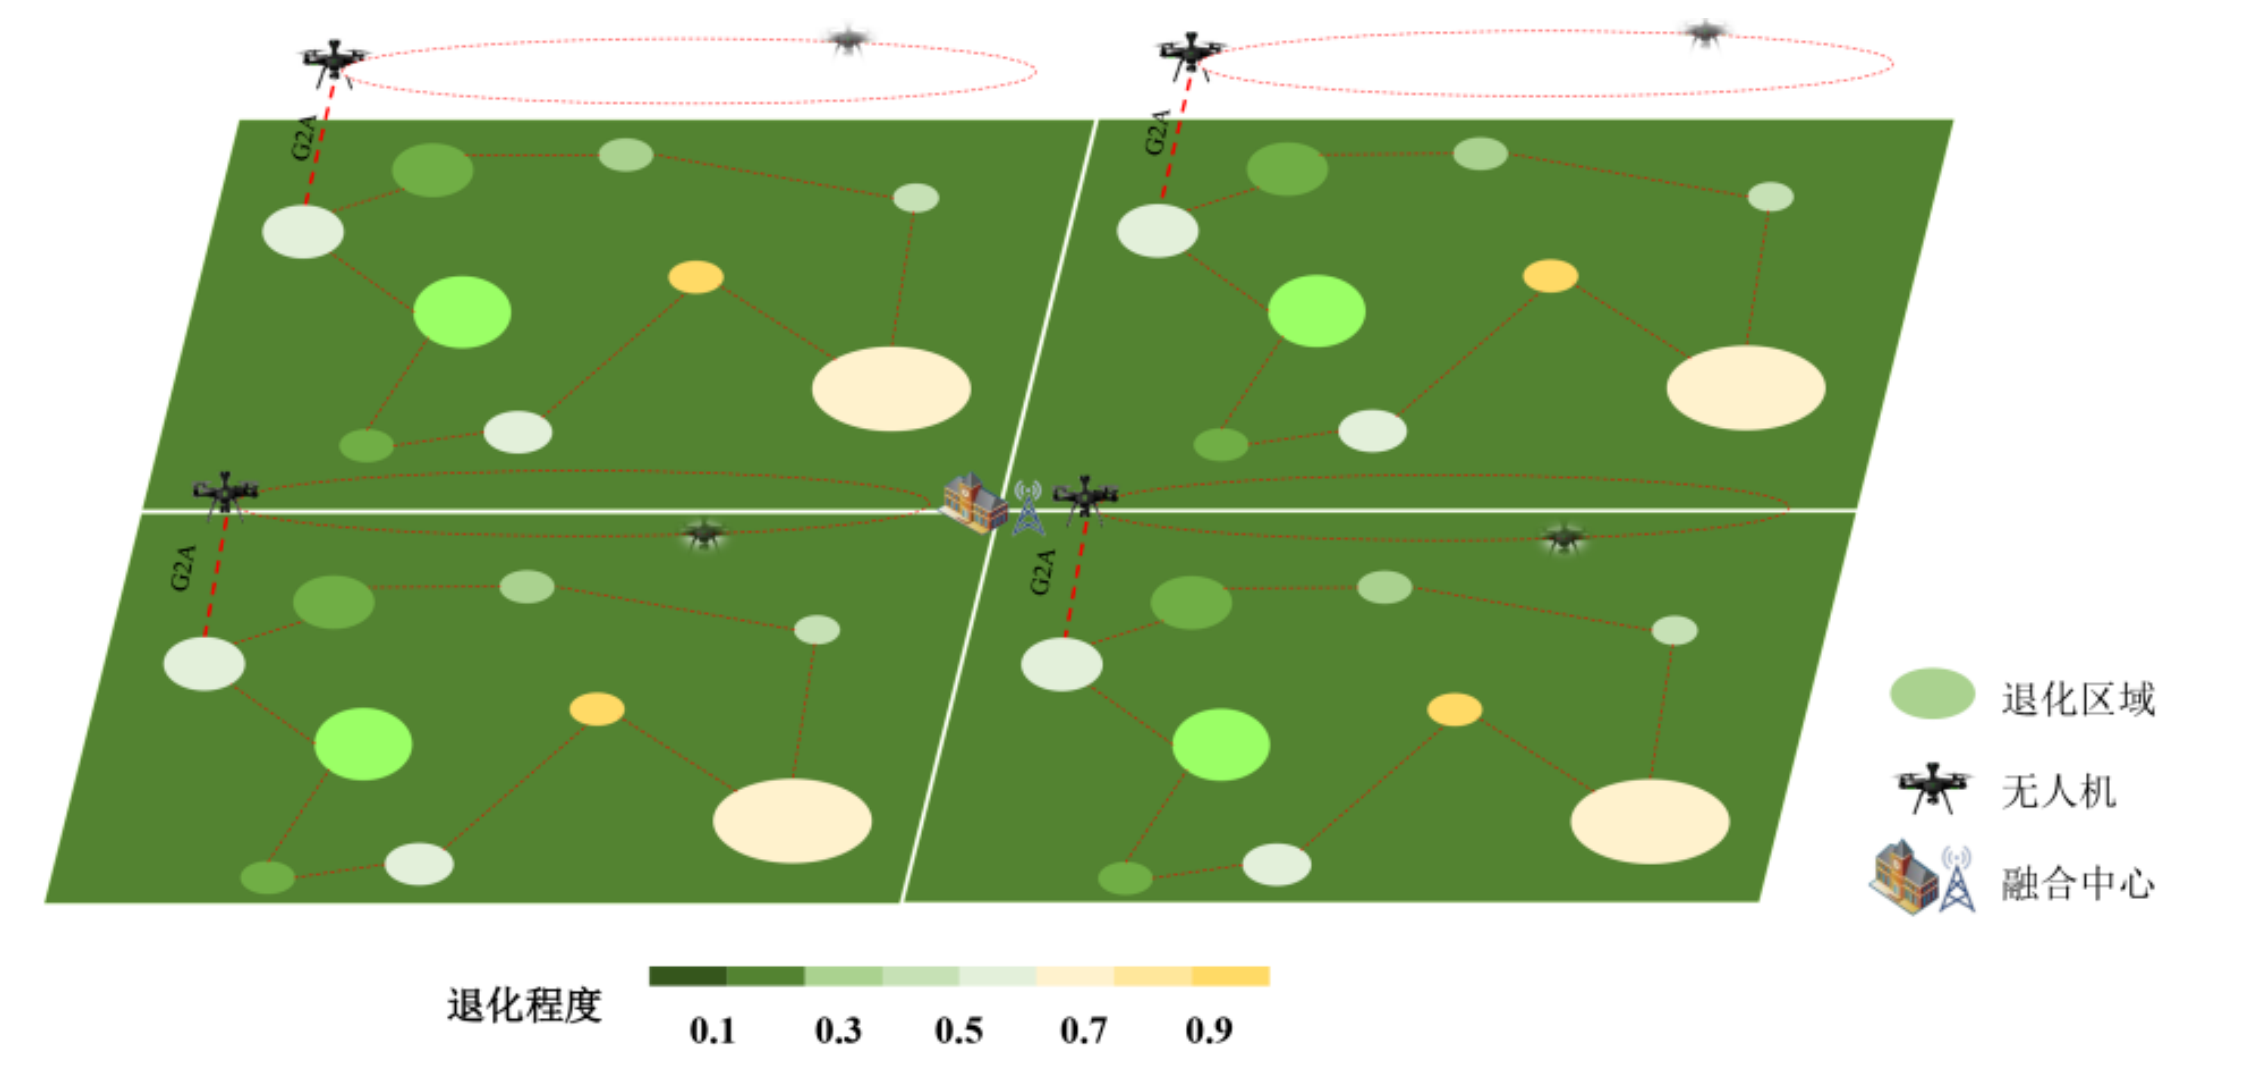
\includegraphics[width=0.7\textwidth]{figures/多无人机修复退化区域实例.png}
	\caption{无人机草原修复区域示意图。图中展示了待修复区域的分布情况,每个圆点代表一个待修复区域,区域大小和颜色深浅表示其退化程度和面积。}
	\label{fig:restored-areas}
\end{figure}

针对待修复草原实例,我们的目标是在无人机从基站出发并在为每个待修复区域提供服务前耗尽能量的情况下,最大化无人机修复的总面积 (假设仅当无人机飞行至待修复区域时才能进行播种)。由于无人机在播撒草籽修复过程中自身重量不断变化,其飞行能耗又与之直接相关,如何权衡无人机飞行能耗与修复能耗之间的关系时问题的核心所在。在修复过程中,无人机的能量消耗主要包括三个部分:无人机在待修复区域中播种的能量消耗、无人机进行航拍的能量消耗以及无人机在飞行过程中的能量消耗。相应地,这三部分能量消耗可以分别表示为 $E_s$, $E_{ap}$ 和 $E_f$。此外,无人机的能量消耗恒定速度下的载荷重量成正比,Dorling\cite{dorling2016vehicle} 等推导出 $h$ 转子无人机的功耗方程,表示如下:


\begin{equation} \label{approximation-power-consumption}
	%\begin{small}
	P(\bar{q}_{ij}) = (M + \bar{q}_{ij})^{\frac{3}{2}}\sqrt{\frac{g^3}{2 \rho \varsigma h}},
	%\end{small}
\end{equation}

其中,$M = W + m$,$W$ 表示无人机框架重量,$m$ 表示其电池重量。$q_{ij}$ 表示无人机当前载荷重量(草籽重量),$g$ 为标准重力加速度,$\rho$ 表示空气密度,$\zeta$ 表示无人机旋转叶片盘面积,$h$ 表示无人机旋翼数量,上述参数单位均参考国际单位制标准。为简化问题,我们假设无人机在待修复区域间以固定高度、恒定速度飞行,同时忽略不同天气条件对无人机飞行的影响,如温度、风力、雨量和沙尘暴等。此外,考虑到无人机能量的限制,我们假设所有草原上的退化区域均可在一次修复过程中由一架无人机修复 (无论是否完全修复)。



\section{各项能量约束}

\subsection{无人机飞行能耗}

无人机飞行期间的能耗,即单架无人机从基站出发,根据修复方案遍历带修复区域最后返回基站的飞行路径能耗。我们设 $x_{ij} \in \{0,1\}$ 为 $0$-$1$ 决策变量,定义如下:

\begin{equation}
	%\begin{small}
	x_{ij} =
	\begin{cases}
		1, & \mbox{$(v_i,v_j)$ is covered in the tour,} \\
		0, & \mbox{otherwise}.
	\end{cases}
	%\end{small}
\end{equation}

我们假定无人机在固定高度以恒定速度 $v$ 飞行,每单位距离的能耗相同。因此修复过程中无人机飞行的总能耗可以表示

\begin{equation} \label{flight-energy}
	\begin{scriptsize}
		E_f =  \sum^N_{i=0}\sum^N_{j \neq i} e^f_{ij} d_{ij} x_{ij},
	\end{scriptsize}
\end{equation}

其中,$e^f_{ij}$ 表示无人机的飞行单位距离的能耗,与无人机在待修复区域 $v_i$ 和 $v_j$ 之间携带的种子重量 $\bar{q}_{ij}$ 相关,可由公式 (1) 实时计算得出。$\bar{q}_{ij}$ 表示从待修复区域 $v_i$ 和 $v_j$ 中无人机携带的草种重量,满足以下条件:

\begin{equation} \label{remained-weight}
	\begin{scriptsize}
		\sum^N_{j=0, i\neq j}\bar{q}_{ji} -  \sum^N_{j=0, i\neq j}\bar{q}_{ij} = Q_i, \forall i \in V_a,
	\end{scriptsize}
\end{equation}
\begin{equation} \label{demanded-weight}
	\begin{small}
		\bar{q}_{ij} \leq Q x_{ij}, \forall (i,j) \in A.
	\end{small}
\end{equation}

\subsection{无人机播种能耗}

我们将每个待修复区域离散为 $c_i(i = 1, ..., n)$ 个单位圆面积。无人机播种的能量消耗可视为与草地退化程度和其携带种子的重量相关的函数。无人机每单位播种面积的能耗可以定义为:$e_i = \eta q_i$。其中 $\eta$ 是一个与能量消耗相关的正参数,$q_i$ 是第 $i$ 个待修复区域每单位圆修复所需种子的重量。进一步地,修复每个区域单位圆面积所需的种子重量可视为该区域的草地退化程度的函数\cite{klaus2017enriching}:$q_i = (1 + l_i) \gamma$。其中,$l_i \in [0.3, 0.8]$ 表示第 $i$ 个待修复区域的草地退化程度,$\gamma$是与草地环境有关的正参数。综上所述,无人机 $u$ 在第 $i$ 个待修复区域中修复 $\sigma_i$ 个单位圆所需的草种重量可以表示为$Q^u_i = \sigma_i q_i$,$\sigma_i$ 表示无人机修复的单位圆数量 $(1\leq\sigma_i\leq c_i)$。因此,无人机 $u$ 在待修复区域内播种的总能量消耗可以表示为:

\begin{equation} \label{seeding-energy}
	\begin{small}
		E_s = \sum^N_{i = 1}\sum^N_{j \neq i}\sigma_i e_i x_{ij},
	\end{small}
\end{equation}

其中,二元 $0-1$ 变量 $x_{ij}$ 用于确定无人机是否将对待修复区域 $v_j$ 进行修复。

\subsection{无人机拍照能耗}

除飞行能耗以外,无人机还在各待修复区域收集修复信息。无人机搭载高光谱相机进行航拍的总能耗可表示为:

\begin{equation} \label{hyper-spectral-camera-energy}
	\begin{scriptsize}
		E_{ap} = e_{ap}\sum^N_{i=1}\sum^N_{j \neq i} x_{ij}\sigma_i,
	\end{scriptsize}
\end{equation}

其中,$e_{ap}$ 表示无人机在 $\sigma_i$ 个被修复的单位圆中航拍所消耗的能量。

\section{1.2 优化目标}

由于能量有限,无人机在一次修复过程中无法修复草原上所有的退化区域。因此,我们的目标是通过无人机技术尽可能多地修复草原的退化面积,即优化目标为:

\begin{equation} \label{maximize-the-sum}
	\begin{small}
		C = \sum^N_{i=1}\sigma_i,
	\end{small}
\end{equation}

\section{问题描述}

综上所述,我们考虑在无人机的最大能量限制 $E_{max}$ 下,对待修复区域的播种修复和航拍能耗 $E_s$ 和 $E_{ap}$、待修复区域间的飞行能耗 $E_f$ 以及无人机的飞行轨迹 $x_{ij}$ 进行组合优化。无人机通过将自身决策与彼此信息实时交流从而实现协同 (修复地图再分配等)。多无人机协同的草原修复模型可被描述为:

\begin{subequations}\label{GRP}
	%\begin{small}
	\begin{align}
		\max_{x_{ij},\sigma_i} \quad & C = \sum^N_{i = 1}\sum^N_{j \neq i} x_{ij}\sigma_i                                                                                                          \\
		\emph{s.t.} \quad            & \sum^N_{i = 1}\sum^N_{j \neq i}\sigma_i e_i x_{ij} + e_{ap}\sum^N_{i=1}\sum^N_{j \neq i} x_{ij}\sigma_i \nonumber                                           \\
		                             & + \sum^N_{i=0}\sum^N_{j \neq i} (M + \bar{q}_{ij})^{\frac{3}{2}}\sqrt{\frac{g^3}{2 \rho \varsigma h}} x_{ij} d_{ij} \leq E_{max}, \label{energy-constraint} \\
		                             & \sum^N_{i=1, i\neq j} \sigma_i q_i x_{ij} \leq Q, \forall j \in V_a,\label{total-load}                                                                      \\
		                             & \sum^N_{j=0, i\neq j}\bar{q}_{ji} -  \sum^N_{j=0, i\neq j}\bar{q}_{ij} = \sigma_i q_i, \label{carry-load} \quad \forall i \in V_a,                          \\
		                             & \bar{q}_{ij} \leq Q x_{ij}, \quad \forall (i,j) \in A, \label{load}                                                                                         \\
		                             & \sum^N_{i=0, i\neq j} x_{ij} = \sum^N_{j=0,i\neq j} x_{ij} = 1, \quad \forall i,j \in V_a, \label{enter-point}                                              \\
		                             & \sum^N_{j=1} x_{0j} = \sum^N_{j=1} x_{j0} = 1, \label{start-point}                                                                                          \\
		                             & x_{ij} \in \{0,1\}, \label{binary-variable}                                                                                                                 \\
		                             & 1 \leq \sigma_i \leq c_i, \label{area-constraint}                                                                                                           \\
		                             & \bar{q}_{ij} \geq 0. \label{flight-weight}
	\end{align}
	%\end{small}
\end{subequations}

% Constraints \eqref{energy-constraint} ensure that the energy consumption in a scheduling cycle of UAV cannot exceed its energy capacity $E_{max}$. Constraints \eqref{total-load} impose that the weight of the grass seeds $Q$ carried by UAV must be sowed before the UAV returns to the base station. Constraints \eqref{carry-load} indicate the reduced weight of grass seeds for UAV after it severs a restored area and equaling the demanded restored area, and also eliminate any illegal subrours. Constraints \eqref{load} guarantee that the demanded grass seeds at the restored area $v_j$ cannot exceed the weight of remaining grass seeds carried by the UAV. Constraints \eqref{enter-point}
% ensure that the UAV enters each restored area at most once and leaves the restored area after seeding.
% Constraints \eqref{start-point}
% guarantee that the UAV begins and ends its route at the base station. Constraint \eqref{binary-variable} ensures that the binary variables value are integers. Constraint \eqref{area-constraint}
% ensures that the number of unit circle to be restored cannot exceed its maximum areas. Constraint \eqref{flight-weight} is  nonnegativity restrictions.

% We can observe that the optimization problem \eqref{GRP} is a multi-variable combinatorial optimization problem, since the set of feasible solutions is discrete in terms of the binary variable $x_{ij}$ and the integer variable $\sigma_i$.
% Therefore, it is difficult to directly solve the optimization problem \eqref{GRP} by using the traditional optimization methods. By further analyzing the optimization problem \eqref{GRP}, we can find the following characteristics. First, the size of restoration areas and the amount of seeding in each restored area may vary with different service order by UAV depending on the UAV's flight trajectory. Second, the size of restoration areas and the amount of seeding in each restored area will affect the next flight trajectory of UAV. In brief, the trajectory design of UAV, the size of restoration areas, and the amount of seeding are closely coupled. If the optimization problem \eqref{GRP} is solved directly, the trajectory design of UAV, the size of restoration areas, and the amount of seeding are generated separately, resulting in that their dependence is ignored unreasonably. Therefore, there exist two challenges for solving effectively the optimization problem \eqref{GRP}.

约束条件 \eqref{energy-constraint} 确保无人机在调度周期内的能耗不超过其最大能量容量 $E_{max}$。约束条件 \eqref{total-load} 要求无人机携带的草种重量 $Q$ 必须在返回基站前完成播种。约束条件 \eqref{carry-load} 规定了无人机在服务恢复区域后草种重量的减少量(等于该区域的需求量),同时消除了任何非法子路径。约束条件 \eqref{load} 保证恢复区域 $v_j$ 所需的草种重量不超过无人机当前携带的剩余草种重量。约束条件 \eqref{enter-point} 确保无人机最多进入每个恢复区域一次,并在播种后离开。约束条件 \eqref{start-point} 要求无人机的路径必须从基站出发并最终返回基站。约束条件 \eqref{binary-variable} 保证二进制变量取整数值。约束条件 \eqref{area-constraint} 规定待恢复的单位圆形区域数量不得超过其最大面积限制。约束条件 \eqref{flight-weight} 则为非负性限制。

可以观察到,优化问题 \eqref{GRP} 是一个多变量组合优化问题,因为其可行解集在二进制变量 $x_{ij}$ 和整数变量 $\sigma_i$ 上是离散的。因此,传统优化方法难以直接求解该问题。通过进一步分析,我们发现以下特征:首先,恢复区域的面积和每个区域的播种量会因无人机服务顺序(即飞行轨迹)的不同而变化;其次,这些参数又会反过来影响无人机的后续飞行轨迹。简而言之,无人机轨迹设计、恢复区域面积和播种量三者紧密耦合。若直接求解优化问题 \eqref{GRP},这三者将被单独生成,导致其依赖关系被不合理忽略。因此,有效求解该问题面临两大挑战。

\chapter{算法求解思路}

\section{基于神经网络的无人机草原修复策略优化}

对于序列决策问题,基于迭代搜索的启发式方法往往能取得能取得较优的效果\cite{feng2015memes}。然而,启发式方法受限于过长的求解时间,同时在一个待修复草原实例下的结果无法迁移,在面对多个待修复草原实例时求解时间往往难以接受。相较之下,神经网络方法以其离线训练、在线决策,泛化能力极强的特性,在面对规模不同、分布各异的序列决策问题时仍然能在极短时间得出较优解,且无需重复训练,因而在组合优化领域广受关注[3]。因此,我们首先提出以单无人机作为智能体,构建深度神经网络模型,利用强化学习方法进行训练,试图学习出一个合理的草原修复策略,以大大节省问题的求解时间。

我们采用强化学习方法相关概念,将无人机视作智能体,其与待修复草原环境的交互过程建模为一个马尔可夫决策过程,如下图所示。智能体的策略建模为神经网络,在与环境的交互中不断收集数据,网络模型通过强化学习Actor-Critic算法进行训练,目标是学习到一个策略$\pi_\theta(a|s)$($\theta$为神经网络参数)使得草原修复面积最大化。

\chapter{基于强化学习的最优修复方案}

\section{马尔可夫过程建模}
我们将修复过程中的每架无人机视为一个智能体,将待修复草原视为以欧几里得距离为边权值的无向全联通图。对单架无人机而言,其部分修复过程可视为从某点出发,遍历修复地图并完成相应修复任务,最后返回起点。

在无人机的修复过程中,由于其在两块相邻修复区域间的飞行能耗正比于此时无人机自身重量与路径长度,而自身重量又随着播散种子修复区域的过程动态变化,因而其总飞行能耗与总飞行长度、修复区域的顺序及修复面积均有复杂关系。换言之,作为优化目标的总修复面积由于与无人机耗能而与其飞行路径间接相关,因而二者之间存在复杂的耦合关系,如何解决修复面积的最优化,毫无疑问是一个困难的 $\text{NP-hard}$ 问题。

针对该难题,我们拟采用强化学习方法学习这一复杂的函数关系,具体建模如下:

\subsection{状态}

本文将一个待修复草原实例设为$V=\{v_i\}_{i=0}^n$,其中包含了各个待修复区域的位置、退化程度等各项信息。各点以$v_0$为起始点按照某种策略$\pi$,逐渐完善部分解$\{(v_0,a_0),(v_i,a_i)\}_{i=1}^{uav_{now}}$。其中,编号$i$表示无人机访问各点的次序,$uav_{now}$为无人机已经过的点数量,$a_i$代表按照策略$\pi$在点$v_i$修复的面积。我们将该部分解作为智能体在强化学习中的状态,记作$s(<i),i\in[1,n+1]$。初始状态记作$s(<1)=v_0$,表示无人机处于地面中心;结束状态记作$s(<n+1)=s$,表示无人机已访问全部点。

\subsection{动作}

如上所述,无人机状态是修复过程的部分解,因而我们将动作设置为无人机修复过程某一步的解,即将无人机在状态$s(<i)$时的动作记作$\pi_i=s(i)$,$i\in[1,n+1]$,即可实现强化学习中动作-状态对的自然更新。

\subsection{状态}

转移函数如上所述,在动作选取完毕后无人机新的状态也被唯一确定,因而状态转移函数具有完全确定性,记其为$S(s(<i)|s(i))=s(<i+1)$,$i\in[1,n]$。

\subsection{策略函数}

如上所述,草原修复过程被创建为一个马尔可夫决策过程,因而其策略函数可被链式分解为:$p(\pi|s)=\prod_{i=1}^n p(s(i)|s(<i))$(10)其中,$p(s(i)|s(<i))$表示智能体在状态$s(<i)$下选择动作$s(i)$的概率。

\subsection{奖励函数}

作为强化学习方法的核心之一,奖励函数的设计必须考虑全面,以防止模型难以收敛。经我们实验证明,单纯以最基本的修复面积作为模型的奖励函数会使得模型收敛速度大大减缓,同时考虑到无人机自身能量限制引入的惩罚项,我们最终将一组解的奖励函数设置为:
\begin{equation}
	R(\pi|V)=\alpha_{p}*Pel+\alpha_{r}*\sum_{i=1}^{n}(l_i-0.3)*a_{i}
	\label{eq:11}
\end{equation}

\begin{equation}
	Pel=\left\{\begin{array}{ll}
		d_{n}^{0}+\sum\limits_{i=1}^{n}d_{i}^{i+1} & E_{rest}<0     \\
		0                                          & E_{rest}\geq 0
	\end{array}\right.
	\label{eq:12}
\end{equation}

上式中,$\alpha_p$, $\alpha_r$为修正系数,$l_i$为第$i$个区域的退化程度,$Pel$为控制无人机能量约束的惩罚项。通过引入$(l_i-0.3)$作为权重因子,模型可以优先修复退化程度更高的区域,从而实现对草原生态健康状况的精准干预。同时为了加快模型收敛速度,我们将不符合无人机能量约束时的惩罚项设置为其从起点到返回地面中心经历的路径长度,以确保在模型收敛的前期尽可能获得的解路径长度较短、符合能量约束,并在此前提下进行修复面积的决策。

\section{神经网络模型构建}

对于序列决策问题,编码器-解码器模型\cite{vaswani2017attention}作为最经典的神经网络模型结构之一,取得了优异的效果。我们采用稍加修改的经典的Tranformer作为编码器,指针网络\cite{vinyals2015pointer}作为自回归解码器以实现构造式求解。

\subsection{特征提取}

我们对待求解的待修复草原模型提取两部分特征,即待修复区域的坐标、退化程度等静态特征,及无人机自身剩余能量、剩余重量等动态特征。静态、动态元素使用各自Transformer作为特征提取器。其中动态元素在构造解的过程中不断变化,需要结合部分解进行循环编码-解码,从而模拟无人机求解过程中负载动态变化的过程,更好地利用无人机当前信息作出更合理的决策。

\subsection{编码器}

参考了Bresson\cite{bresson2021transformer}等人的方法。编码器结构如图3所示,由$L$层堆叠而成,采取BatchNorm归一化,公式可表示为:

\begin{equation}
	h^{l=0} = h^{in} W^{in} \in \mathbb{R}^{n \times d}
	\label{eq:13a}
\end{equation}

\begin{equation}
	h_{rc}^{l+1} = \text{BN}\left(\text{MHA}^{l+1}(h^l) + h^l\right)
	\label{eq:13b}
\end{equation}

\begin{equation}
	h^{l+1} = \text{BN}\left(\text{Relu}\left(h_{rc}^{l+1} W_1^{l+1}\right) W_2^{l+1} + h_{rc}^{l+1}\right)
	\label{eq:13c}
\end{equation}

\subsection{解码器}

自回归解码器的作用是循环解码以逐步实现解的构造。首先输入静态、动态编码器的输出作为输入,通过注意力机制选择出第一个结点,然后利用循环神经网络学习已选择的结点信息更新解嵌入,再通过注意力机制选择下一个待修复区域及修复面积,以此类推直至所有结点[14]。

具体而言,解码器的输入有:静态特征、动态特征、访问的上一个结点的隐藏特征。开始时上一个结点的隐藏特征初始化为全零向量,之后每次决策出下一个待修复区域及修复面积后,对解码器输入的动态元素及掩码进行更新以剔除不可行结点及修复方案。



\begin{equation}
	rm^{i}, h_{gru}^{i} =
	\left\{
	\begin{array}{ll}
		GRU(h_{0}^{i}, 0)               & i = 0 \\
		GRU(h_{i-1}^{i}, h_{gru}^{i-1}) & i > 0
	\end{array}
	\right.
	\label{eq:14}
\end{equation}

其中,$0$为全零向量,$GRU$(gated recurrent unit)为循环神经网络更新解嵌入,$h_i^{i-1}$为上一轮选择结点的结点嵌入。

自回归解码器接收上述输入后,先对所有输入做一次自注意力以进一步聚集所有结点的嵌入,而后通过两次线性聚合层得到当前修复地图的全局信息上下文并将其与当前局部信息相结合,以得出各个到达待修复区域$i$修复相应大小区域$a_i$的概率$p(i|s_i)$(二维)。同时,我们需要将解码器输出的概率进行一次掩码操作以过滤掉所有之前以到达过的待修复区域及各修复区域中不合法的修复面积方案。

\begin{equation}
	h_{p}^{l=i} = \text{Attention}(\text{static}, \text{dynamic}^{i}, mn^{i})
	\label{eq:15a}
\end{equation}

\begin{equation}
	\mu_{i} =
	\begin{cases}
		C \times \text{Tanh}\left((W_{q}h_{p}^{l=i})^{T}(W_{k}h_{p}^{l=i})\right) & x_{i} \notin \pi_{i} \\
		-\infty                                                                   & \text{otherwise}
	\end{cases}
	\label{eq:15b}
\end{equation}

\begin{equation}
	p(i|s_{i}) = \text{Softmax}(\mu_{i})
	\label{eq:15c}
\end{equation}

其中,$W_q,W_k\in\mathbb{R}^{d\times d}$为可学习参数矩阵。我们通过掩码设置$\mu_i=-\infty$以避免重复选择结点,每次选择对应结点(即待修复区域)及修复面积后,对解码器输入的动态元素及掩码进行更新以剔除不可行结点及修复方案。

\section{模型训练}
对于建立的单无人机修复模型,我们采用强化学习Actor-Critic算法\cite{sutton1999policy}进行梯度更新。模型中作为主体的Actor网络用于近似草原修复过程中的策略概率函数p(π|s),记其网络参数为θ,则网络的待优化目标可表示为:

\begin{equation}
	J(\theta \mid s) = \mathbb{E}_{t \sim p_{\theta(\cdot | V)}} R(\pi \mid s)
	\label{eq:16}
\end{equation}

我们参考了Williams等的方法\cite{williams1992simple},将上述策略梯度函数表示为:

\begin{align}
	\nabla_{\theta}J(\theta \mid s)
	 & = \mathbb{E}_{t \sim p_{\theta}(\cdot \mid s)} \left[(R(\pi \mid s) - b(s)) \nabla_{\theta} \ln p_{\theta}(\pi \mid s)\right] \label{eq:17a} \\
	 & = \mathbb{E}_{t \sim p_{\theta}(\cdot \mid s)} \left[A(\pi \mid s) \nabla_{\theta} \ln p_{\theta}(\pi \mid s)\right] \label{eq:17b}
\end{align}
其中,$R(\pi|s)$代表草原修复过程中计算得的奖励值;动作概率$p_\theta(\pi|s)$代表Actor网络在草原修复过程中每次自回归时选择修复区域及修复面积大小的概率;$b(s)$为REINFORCE算法[17]中的基线函数,即Critic网络输出的估计值;$A(\pi|s)=R(\pi|s)-b(s)$为优势函数,表示在状态$s$下策略$\pi$的优劣,乘以$\nabla_\theta\ln p_\theta(\pi|s)$,表示若优势函数$A(\pi|s)$为正数则增大概率,若为负数则减小概率。

若设训练的图批次大小为$B$,每张图中点集大小为$L$,每次训练都按照策略函数$p_\theta(\pi|s)$从各图中抽取一组可能的解,则Actor网络梯度可近似为:

\begin{equation}
	\nabla_{\theta} J(\theta \mid s) \approx \frac{1}{B} \sum_{i=1}^{B} \sum_{j=1}^{L} \left[ A(\pi_j \mid s_j) \nabla_{\theta} \ln p_{\theta}(\pi_j \mid s_j) \right]
	\label{eq:18}
\end{equation}

将Critic网络参数设为$\theta_c$,则Critic网络优化目标可近似为:

\begin{equation}
	L(s) = \frac{1}{B} \sum_{i=1}^{B} \left( R(V_i) - R_w(V_i) \right)^2
	\label{eq:19}
\end{equation}

模型的具体训练过程如下算法$3$所示。算法通过在每个$epoch$内随机生成实例用于对网络进行训练与验证。通过指针网络的自回归性质构造性地得到当前策略下实例的解,并将其作为下一次网络的输入直至得到完整的解。根据公式计算得到相应的优势函数值后,通过$Adam$($adaptive$ $moment$ $estimation$)优化器\cite{kingma2014adam}对$Actor$-$Critic$网络进行参数更新,其中基线函数$b(s)$为$Critic$网络对当前实例估计的奖励值。

% %\vspace{-0.10in}
% \begin{algorithm}[h]
% 	\begin{algorithmic}[1]
% 		\caption{Actor-Critic 网络训练算法} \label{alg:actor_critic}
% 		\Require Actor-Critic 网络所有参数 $\theta_c$、$\theta_e$,学习率 $\alpha$,训练回合数 $N_{epoch}$,训练集大小 $B_T$,验证集大小 $B_V$,训练批次 $B$,训练序列长度 $L$,训练序列面积上限 $area_{max}$ 及 $area_{min}$
% 		\Ensure 收敛的神经网络参数 $\theta_c$、$\theta_e$

% 		\State $i_{epoch} \leftarrow 0$
% 		\While{$i_{epoch} < N_{epoch}$}
% 		\State 随机生成规模为 $B_T$ 的训练集 $train\_set$ 及规模为 $B_V$ 的验证集 $valid\_set$,将训练集分割为 $\lceil \frac{B_T}{B} \rceil$ 份
% 		\State $t_e \leftarrow 0$
% 		\For{$t_e$ to $\lceil \frac{B_T}{B} \rceil$}
% 		\State 取训练集中第 $t_e$ 份作为 $T_{data}$
% 		\State $i_{steps} \leftarrow 0$
% 		\State Initial(mask) \Comment{初始化 mask 掩码}
% 		\State Initial(resolution) \Comment{初始化解的存储空间}
% 		\While{$i_{steps} < L$}
% 		\State $(ptr, area) \leftarrow \text{Actor}(T_{data})$ \Comment{Actor 网络输出部分解}
% 		\While{Mask(ptr, area, mask)}
% 		\State $(ptr, area) \leftarrow \text{Actor}(T_{data})$ \Comment{屏蔽求解过程中非法的解}
% 		\EndWhile
% 		\State Update(mask)
% 		\State Update(resolution, $(ptr, area)$)
% 		\State $i_{steps} \leftarrow i_{steps} + 1$
% 		\EndWhile
% 		\State $R \leftarrow \text{Reward}(resolution, T_{data})$ \Comment{根据公式计算当前策略获得的奖励值}
% 		\State $b \leftarrow \text{Critic}(T_{data})$ \Comment{根据公式计算 Critic 网络的基线估计值}
% 		\State $A \leftarrow \|R - b\|_2^2$ \Comment{计算优势函数值}
% 		\State $\nabla\theta \leftarrow \text{Loss}(resolution, A)$ \Comment{计算网络梯度}
% 		\State $\theta, \theta_e \leftarrow \text{Adam}(\theta, \theta_e, \alpha, \nabla\theta)$
% 		\EndFor

% 		\If{$i_{epoch} == 0$}
% 		\State $\theta^* \leftarrow \theta$
% 		\Else
% 		\If{$\text{Reward}(\text{Valid}(\theta, valid\_set)) > \text{Reward}(\text{Valid}(\theta^*, valid\_set))$}
% 		\State $\theta^* \leftarrow \theta$
% 		\EndIf
% 		\EndIf
% 		\State $i_{epoch} \leftarrow i_{epoch} + 1$
% 		\EndWhile
% 	\end{algorithmic}
% \end{algorithm}


\begin{algorithm}[h] \begin{algorithmic}[1] \caption{Attention Model Training Algorithm for GRP} \label{alg:grp_training} \Require $\theta \in \Theta$ (model parameters), $d_e \in \mathbb{N}$ (embedding dimension), $d_h \in \mathbb{N}$ (hidden dimension), $n_{layers} \in \mathbb{N}$ (encoder layers), $n_{heads} \in \mathbb{N}$ (attention heads), $\alpha \in \mathbb{R}^{+}$ (learning rate), $N_{epoch} \in \mathbb{N}$ (training epochs), $B \in \mathbb{N}$ (batch size), $G_{size} \in \mathbb{N}$ (graph size), $B_{type} \in {\text{None}, \text{Exponential}, \text{Critic}, \text{Rollout}}$ (baseline type) \Ensure $\theta^* \in \Theta$ (optimal parameters)
		\State $M_{\theta} \leftarrow \text{InitializeModel}(d_e, d_h, n_{layers}, n_{heads}, \theta)$
		\State $B_{model} \leftarrow \text{InitializeBaseline}(B_{type})$
		\State $\mathcal{O} \leftarrow \text{Adam}(\{M_{\theta}, B_{model}\}, \alpha)$
		\State $\mathcal{S} \leftarrow \text{LRScheduler}(\alpha)$
		\State $\mathcal{D}_{val} \leftarrow \{x_i\}_{i=1}^{val\_size}$ \Comment{Generate validation dataset}

		\State $R_{best} \leftarrow -\infty$ \Comment{Best reward tracker}
		\For{$e = 0$ \textbf{to} $N_{epoch} - 1$}
		\State $\mathcal{D}_{train} \leftarrow \{x_i\}_{i=1}^{epoch\_size}$ \Comment{Generate training dataset}
		\State $\{\mathcal{B}_j\}_{j=1}^{n_B} \leftarrow \text{BatchSplit}(\mathcal{D}_{train}, B)$ where $n_B = \lceil\frac{|\mathcal{D}_{train}|}{B}\rceil$
		\State $M_{\theta} \leftarrow M_{\theta}.\text{train}()$ \Comment{Set model to training mode}
		\State $M_{\theta}.\text{decode\_type} \leftarrow \text{"sampling"}$

		\For{$\mathcal{B} \in \{\mathcal{B}_j\}_{j=1}^{n_B}$}
		\State $(x, b_v) \leftarrow B_{model}.\text{unwrap\_batch}(\mathcal{B})$
		\State $x \leftarrow x.\text{to}(\text{device})$, $b_v \leftarrow b_v.\text{to}(\text{device})$ if $b_v \neq \text{None}$ else $\text{None}$

		\State \textcolor{blue}{// Forward pass}
		\State $(C, \log p) \leftarrow M_{\theta}(x)$ \Comment{$C \in \mathbb{R}^{B}$: costs, $\log p \in \mathbb{R}^{B \times L}$: log-probabilities}
		\State $r \leftarrow -C$ \Comment{$r \in \mathbb{R}^{B}$: rewards}

		\State \textcolor{blue}{// Extract GRP-specific metrics}
		\If{$\text{problem\_type} = \text{"grp"}$}
		\State $A_{repair} \leftarrow \begin{cases}
				x.\text{total\_repair\_area} & \text{if exists}                 \\
				-C / \alpha_{r}              & \text{otherwise (approximation)}
			\end{cases}$
		\EndIf

		\State \textcolor{blue}{// Evaluate baseline value}
		\State $(b_v, \mathcal{L}_{b}) \leftarrow \begin{cases}
				B_{model}.\text{eval}(x, C) & \text{if } b_v = \text{None} \\
				(b_v, 0)                    & \text{otherwise}
			\end{cases}$

		\State \textcolor{blue}{// Compute REINFORCE loss}
		\State $\mathcal{L}_{R} \leftarrow \frac{1}{B}\sum_{i=1}^{B}(C_i - b_{v,i}) \cdot \log p_i$ \Comment{REINFORCE loss}
		\State $\mathcal{L} \leftarrow \mathcal{L}_{R} + \mathcal{L}_{b}$ \Comment{Total loss}

		\State \textcolor{blue}{// Backpropagation and parameter update}
		\State $\nabla\theta \leftarrow \mathbf{0}$ \Comment{Zero gradients}
		\State $\nabla\theta \leftarrow \nabla_{\theta}\mathcal{L}$ \Comment{Compute gradients}
		\State $\|\nabla\theta\|_2 \leftarrow \min(\|\nabla\theta\|_2, g_{max})$ \Comment{Clip gradient norm}
		\State $\nabla\theta \leftarrow \begin{cases}
				0            & \text{if } \nabla\theta \in \{\text{NaN}, \pm\infty\} \\
				\nabla\theta & \text{otherwise}
			\end{cases}$ \Comment{Fix invalid gradients}
		\State $\theta \leftarrow \mathcal{O}(\theta, \nabla\theta)$ \Comment{Update parameters}
		\EndFor

		\State \textcolor{blue}{// Validation phase}
		\State $M_{\theta}.\text{decode\_type} \leftarrow \text{"greedy"}$
		\State $M_{\theta} \leftarrow M_{\theta}.\text{eval}()$
		\State $C_{val} \leftarrow \text{Evaluate}(M_{\theta}, \mathcal{D}_{val})$ \Comment{$C_{val} \in \mathbb{R}^{|\mathcal{D}_{val}|}$}
		\State $\bar{r} \leftarrow -\frac{1}{|\mathcal{D}_{val}|}\sum_{i=1}^{|\mathcal{D}_{val}|} C_{val,i}$ \Comment{Average reward}

		\State $B_{model} \leftarrow B_{model}.\text{epoch\_callback}(M_{\theta}, e)$ \Comment{Update baseline}
		\State $\alpha \leftarrow \mathcal{S}(\alpha)$ \Comment{Update learning rate}

		\If{$e \bmod k_{save} = 0 \lor e = N_{epoch} - 1$}
		\State $\text{SaveCheckpoint}(\theta, \mathcal{O}, B_{model}, e)$
		\EndIf

		\If{$e = 0 \lor \bar{r} > R_{best}$}
		\State $\theta^* \leftarrow \theta$
		\State $R_{best} \leftarrow \bar{r}$
		\EndIf
		\EndFor

		\State \Return $\theta^*$
	\end{algorithmic}
\end{algorithm}

\chapter{多无人机协同调度算法}

假设各无人机每轮巡航所携带的种子数量相同,在修复过程中无人机自身重量因种子播撒而减轻,因而导致其能飞行能耗变化,无人机已知自身修复地图的详细信息(退化区域的数量及区域位置、退化程度及待修复面积等退化区域信息),距离计算采用二维平面内的欧式距离公式。

本文考虑了一种多无人机协同调度算法,该算法通过单个无人机的局部信息和中心汇总的全局信息来实现多个无人机之间的协同。在算法的输入部分,除了对参数进行设定外,本文还需要为每架无人机初始化修复地图$M$及记录无人机信息的状态集$S$。$M$中涵盖了每架无人机的待修复任务点,每个任务点包含有任务点编号、坐标的位置、退化程度以及可修复面积;$S$中则记录无人机当前的位置、剩余能量、已访问序列和已修复面积。同时,为了模拟无人机与地面中心交互的先后顺序,我们引入信号量这一机制以确保无人机与地面中心交流的通畅,该信号量定义为无人机在当前修复地图下最先完成首个待修复区域目标的时间,故其与无人机前往下一个区域的飞行时间与修复时间直接相关。

而在算法的输出部分,算法结束后应由中心对无人机状态集合$S$进行汇总,输出各无人机的访问序列、修复面积及剩余能量,以便对算法进行分析。

简而言之,该设计的多无人机协同算法主要思想是动态调整无人机修复地图,通过适应度函数 $\Theta(uav,M_u)$(如最短路径函数等)在修复过程中结合无人机自身位置等信息再分配地图以期望得到一个更好的结果。

无人机从地面控制中心出发,其初始修复地图可按照K-means等聚类方法划分,首先前往修复地图中适应度函数最小(如距离)的结点。随后,各无人机以当前位置为出发点,按照修复地图进行第一次最优路径规划;并计算该方案下,去除完成本路径及返航的飞行能耗、在剩余各点(包含当前点)进行信息收集的能耗及修复一单位面积所需要的能耗后,本机修复的面积。此处要特别说明,无人机在路径规划中通过循环确保得出的解一定符合能力约束要求,即按照某一路径规划方案,依次访问每个点,并完成信息采集与至少1单位面积的修复工作后,仍然剩余的能量大于0。

无人机记录本次的规划方案,并将当前的修复地图、自身位置、修复面积等信息上报中心。中心汇总各无人机的修复地图得到全局修复地图,剔除其中每个无人机当前所在点;中心依次遍历地图中各点,根据已知信息,结合适应度函数 $\Theta(uav,M_u)$ 寻找与其最适合的无人机,并将该点加入对应无人机的新地图中。完成地图更新后,中心将新地图下发给各无人机。信号量最大的无人机以当前位置为出发点,按照调整过的新修复地图进行第二次最优路径规划,并计算该方案下的修复面积。对本次的规划方案做好记录后,并将第二次规划中的修复面积等信息上报中心。中心汇总上报信息,计算第二次的多机体系总修复面积;中心将两次修复面积进行比较,若第一次大于等于第二次,则新地图作废,反之,用新地图替代旧地图;中心将最终决策下达各无人机。无人机根据中心决策判断是否更新地图,并选择地图对应的剩余能量和规划方案。信号量最大的无人机在当前点完成信息采集和面积修复工作后,按照规划方案前往下一个点,并将当前点加入已访问序列,同时更新自身信号量。

重复上述决策过程,当某架无人机的修复地图为空时,该无人机返回中心,并在此后不再参与无人机群同中心的交互;当全局修复地图为空时(全部无人机返航),该算法结束。

\begin{algorithm}[H]
	\caption{多元人机协同调度算法}
	\label{alg:multi_uav_scheduling}
	\begin{algorithmic}[1]
		\Require 参数序列 $Parms$,无人机修复地图集合 $M_u$,无人机状态集合 $S_u$
		\Ensure 无人机访问的节点序列 $O_p$,无人机修复的面积 $O_a$,无人机剩余能量 $O_e$

		\State $M_u^i \gets \text{Initial}(M_u)$ \Comment{无人机根据初始化方法(如 K-means)分配初始地图}
		\State $P_u^i \gets \text{Initial}(P_u)$ \Comment{初始化无人机信号量以决定决策优先级}

		\While{$M_u \neq \emptyset$}
		\State $E_u^{rel} \gets \text{PlaningPath}(M_u, P_u^{self})$ \Comment{无人机群第一次路径规划}
		\State $\text{SendToCenter}(S_u, M_u, E_u^{rel})$ \Comment{无人机第一次上报中心}
		\State $M_u^{tmp} \gets \text{updateMap}(M^{global}, P_u^{self})$ \Comment{中心更新地图}
		\State $\text{RecvToUAV}(M_u^{P_u^{tmp}})$ \Comment{中心给无人机下发新地图}
		\State $E_u^{r2} \gets \text{PlaningPath}(M_u^{tmp}, P_u^{self})$ \Comment{无人机群第二次路径规划}
		\State $\text{SendToCenter}(E_u^{r2}, Area_u^{r2})$ \Comment{无人机第二次上报中心}

		\If{$\sum_{u=1}^U Area_u^{r2} \geq \sum_{u=1}^U Area_u^{r1}$}
		\State $\text{RecvToUAV}(M_u^{tmp})$ \Comment{无人机选择修复面积更多的地图}
		\State $M_u \gets M_u^{tmp}$
		\EndIf

		\State $\sigma_u^{max\_p} \gets \text{DecideArea}(E_u, M_u)$ \Comment{信号量最优先的无人机决策修复面积}
		\State $\text{ActionUAV}(\sigma_u^{max\_p}, C_{max\_p}, P_u^{max\_p})$ \Comment{无人机执行修复和信息采集}
		\State $\text{DropPointFromMap}(M_u, P_u^{max\_p})$
		\State $P_u^{max\_p} \gets \text{FlyToPoint}(P_u^{benefit})$ \Comment{无人机飞往下个最优点}
		\State $\text{Update}(P_u^{max\_p})$ \Comment{更新无人机信号量}
		\EndWhile

		\State $\text{FlyToPoint}(P_u^0)$ \Comment{无人机返回起点}
	\end{algorithmic}
\end{algorithm}


\chapter{实验与分析}
本部分我们展示了一些仿真实验的具体配置与结果。
\label{sub:实验配置表格}
\section{仿真配置}
\begin{table}[H]
	\centering
	\caption{实验硬件配置}
	\begin{tabular}{ll} % 使用两列左对齐格式
		\toprule
		配置      & 描述                                                       \\
		\midrule
		CPU     & AMD Ryzen Threadripper 3970X 32-Core Processor, 3.79 GHz \\
		GPU     & NVIDIA GeForce RTX 3090 Ti                               \\
		RAM     & ADATA 192GB-DDR4                                         \\
		OS      & Ubuntu Server 22.04.3 LTS                                \\
		Python  & Python 3.9                                               \\
		PyTorch & version 1.12.1+cu113                                     \\
		\bottomrule
	\end{tabular}
	\label{tbl_hardware_config}
\end{table}
\section{实例设置}
为验证所提出模型与算法的有效性,本文在六种不同规模的草原实例上进行了仿真,草原区域边长分别为 $500$ 到 $1000$,步长为 $100$。所有实例均在二维空间内定义,任意两个待修复区域 $v_i$ 与 $v_j$ 之间的距离采用欧氏距离计算。每组实例中,待修复区域数量 $N$ 分别设置为 $60, 80, 100, 120, 140, 160$,无人机数量 $U$ 设置为 $4, 6, 8$,单架无人机的活动范围 $L$ 与草原边长一致。所有待修复区域的坐标均在对应草原区域内随机生成,退化程度 $l_i$ 服从 $[0.3, 0.8]$ 的均匀分布,基站均位于 $(0,0)$。每个待修复区域的最大可修复单位圆数量 $\sigma_i$ 随区域面积变化,范围为 $10$ 到 $35$,步长为 $5$。无人机初始能量 $E_{max}$ 与草原规模对应,具体参数如表\ref{tbl_instance_setting} 所示。

\begin{table}[H]
	\centering
	\caption{仿真实验实例设置参数表}
	\begin{tabular}{lll}
		\toprule
		参数  & 描述       & 值                               \\
		\midrule
		$N$ & 待修复区域数量  & $60, 80, 100, 120, 140, 160$    \\
		$U$ & 无人机数量    & $4, 6, 8$                       \\
		$L$ & 单无人机活动范围 & $500, 600, 700, 800, 900, 1000$ \\
		\bottomrule
	\end{tabular}
	\label{tbl_instance_setting}
\end{table}

\section{算法对比设置}

为了与研究热点中的最优化路径规划策略\cite{aggarwal2020path}进行比较,我们设置了如下对比算法:

\textbf{协同启发式与概率模型学习算法(CHAPBILM)\cite{JIAO2024108084}}:该方法将问题分解为两阶段,第一阶段采用启发式算法(如2-opt、or-opt等)优化无人机的访问顺序,第二阶段利用概率模型学习(PBIL)动态分配各区域的修复面积,并结合最大剩余能量局部搜索(MRELS)进一步提升解的质量。该方法通过协同优化路径和修复面积,充分考虑了两者的耦合关系,提升了整体修复效果。

该算法可与多无人机协同调度算法结合,进一步验证我们提出方法的有效性和优越性。
\section{参数设置}
实验仿真具体参数如下。

\label{sub:无人机参数表格}
\begin{table}[H]
	\centering
	\caption{实验软件配置}
	\begin{tabular}{lll} % 三列左对齐格式
		\toprule
		参数              & 描述                & 值                   \\
		\midrule
		\( M \)         & 无人机重量             & 1.5                 \\
		\( g \)         & 重力加速度             & 9.8                 \\
		\( \rho \)      & 空气流体密度            & 1.024               \\
		\( \zeta \)     & 无人机旋转螺旋桨面积        & 0.2                 \\
		\( h \)         & 无人机旋翼数            & 6                   \\
		\( \gamma \)    & 修复能耗正系数           & 2                   \\
		\( \eta \)      & 草原环境相关的正系数        & \( 1 \times 10^4 \) \\
		\( e_{ap} \)    & 无人机收集一个单位圆信息所需的能耗 & \( 2 \times 10^4 \) \\
		\( E_{max} \)   & 无人机所携带的最大能量       & \( 3 \times 10^6 \) \\
		\( B \)         & 强化学习模型训练时的图批次大小   & 512                 \\
		\( N_{epoch} \) & 强化学习模型训练时的回合数     & 512                 \\
		\bottomrule
	\end{tabular}
	\label{tbl_drone_parameters}
\end{table}

\section{仿真结果}


下面我们展示本文所提出方法的仿真实验结果,包括训练过程中的损失函数和修复面积变化曲线,以及不同方法的路径规划可视化对比结果。

\begin{figure}[H]
	\centering
	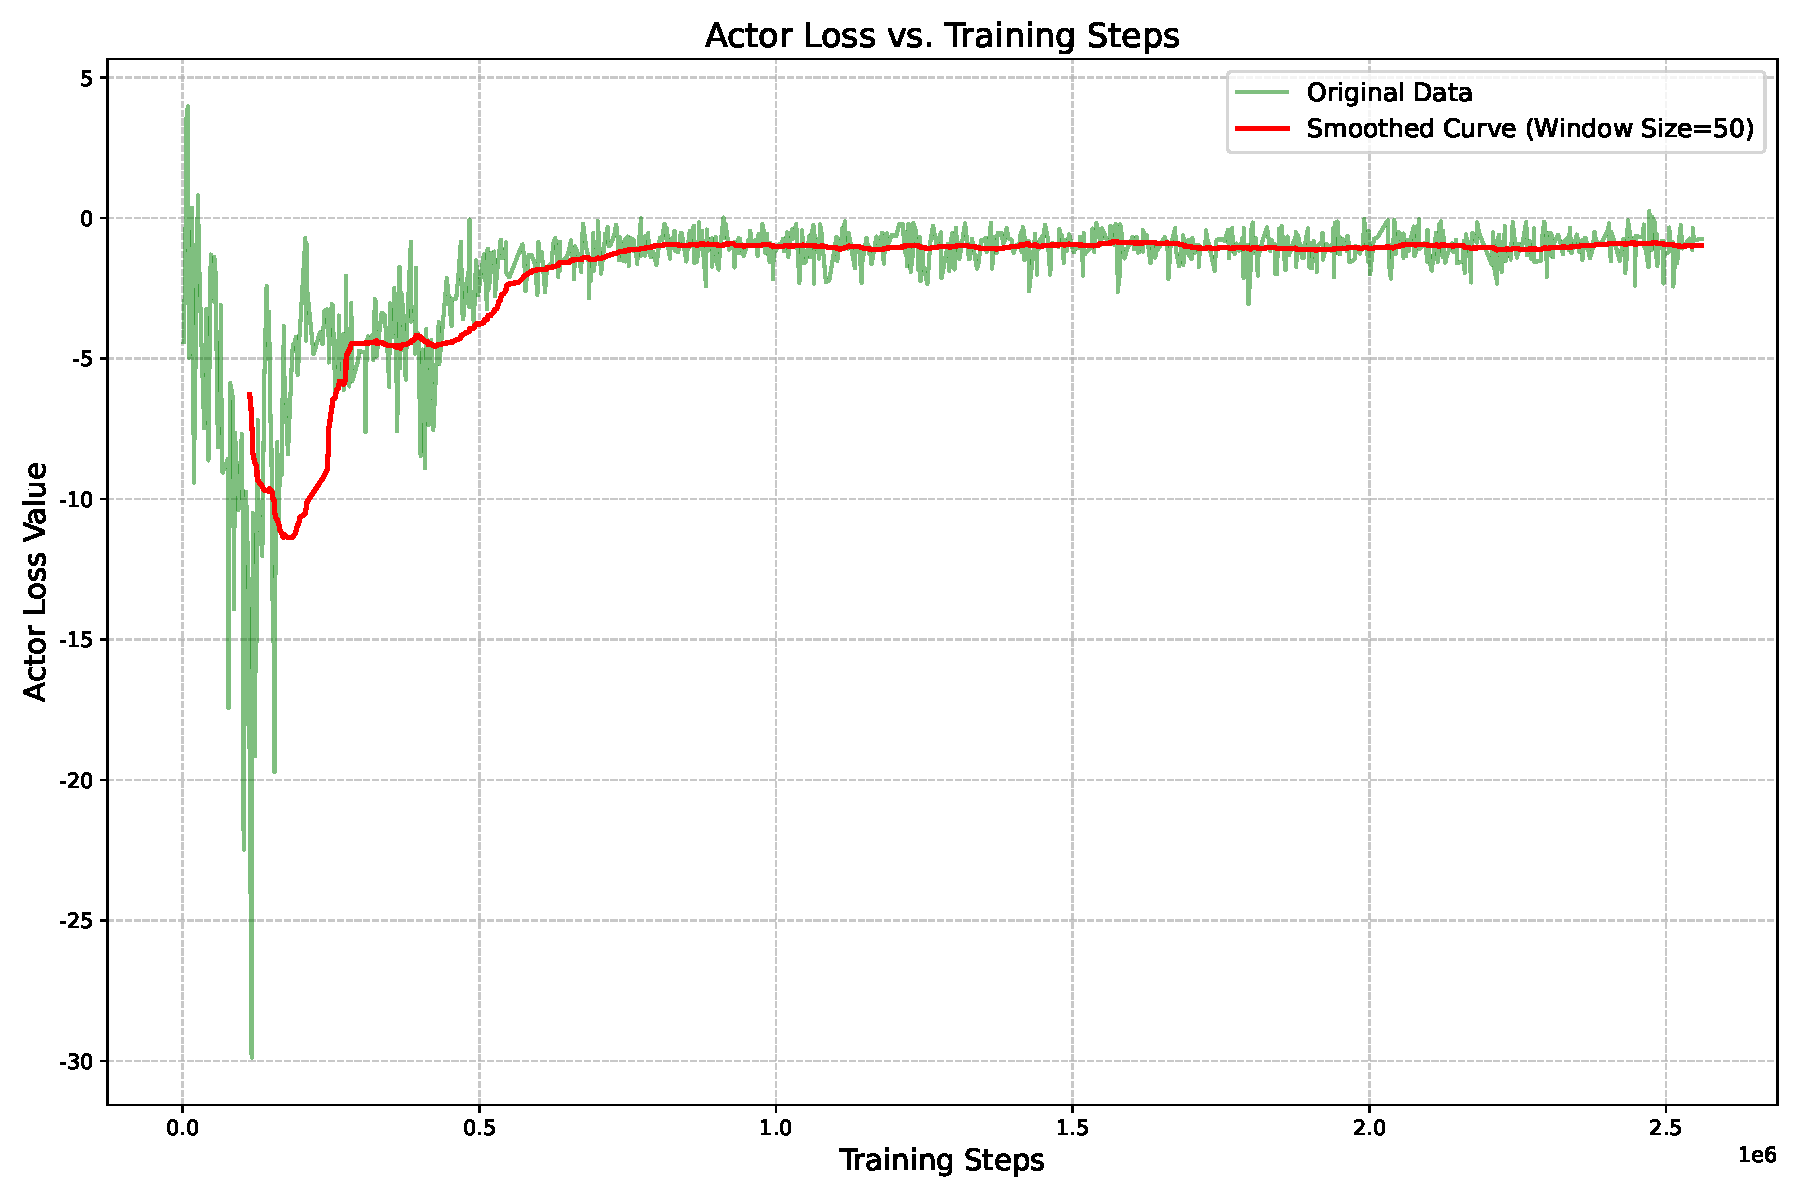
\includegraphics[width=0.6\textwidth]{figures/actor_loss_curve.pdf}
	\caption{深度强化学习训练过程中的损失函数变化}
	\label{fig:training_loss_curve}
\end{figure}

\begin{figure}[H]
	\centering
	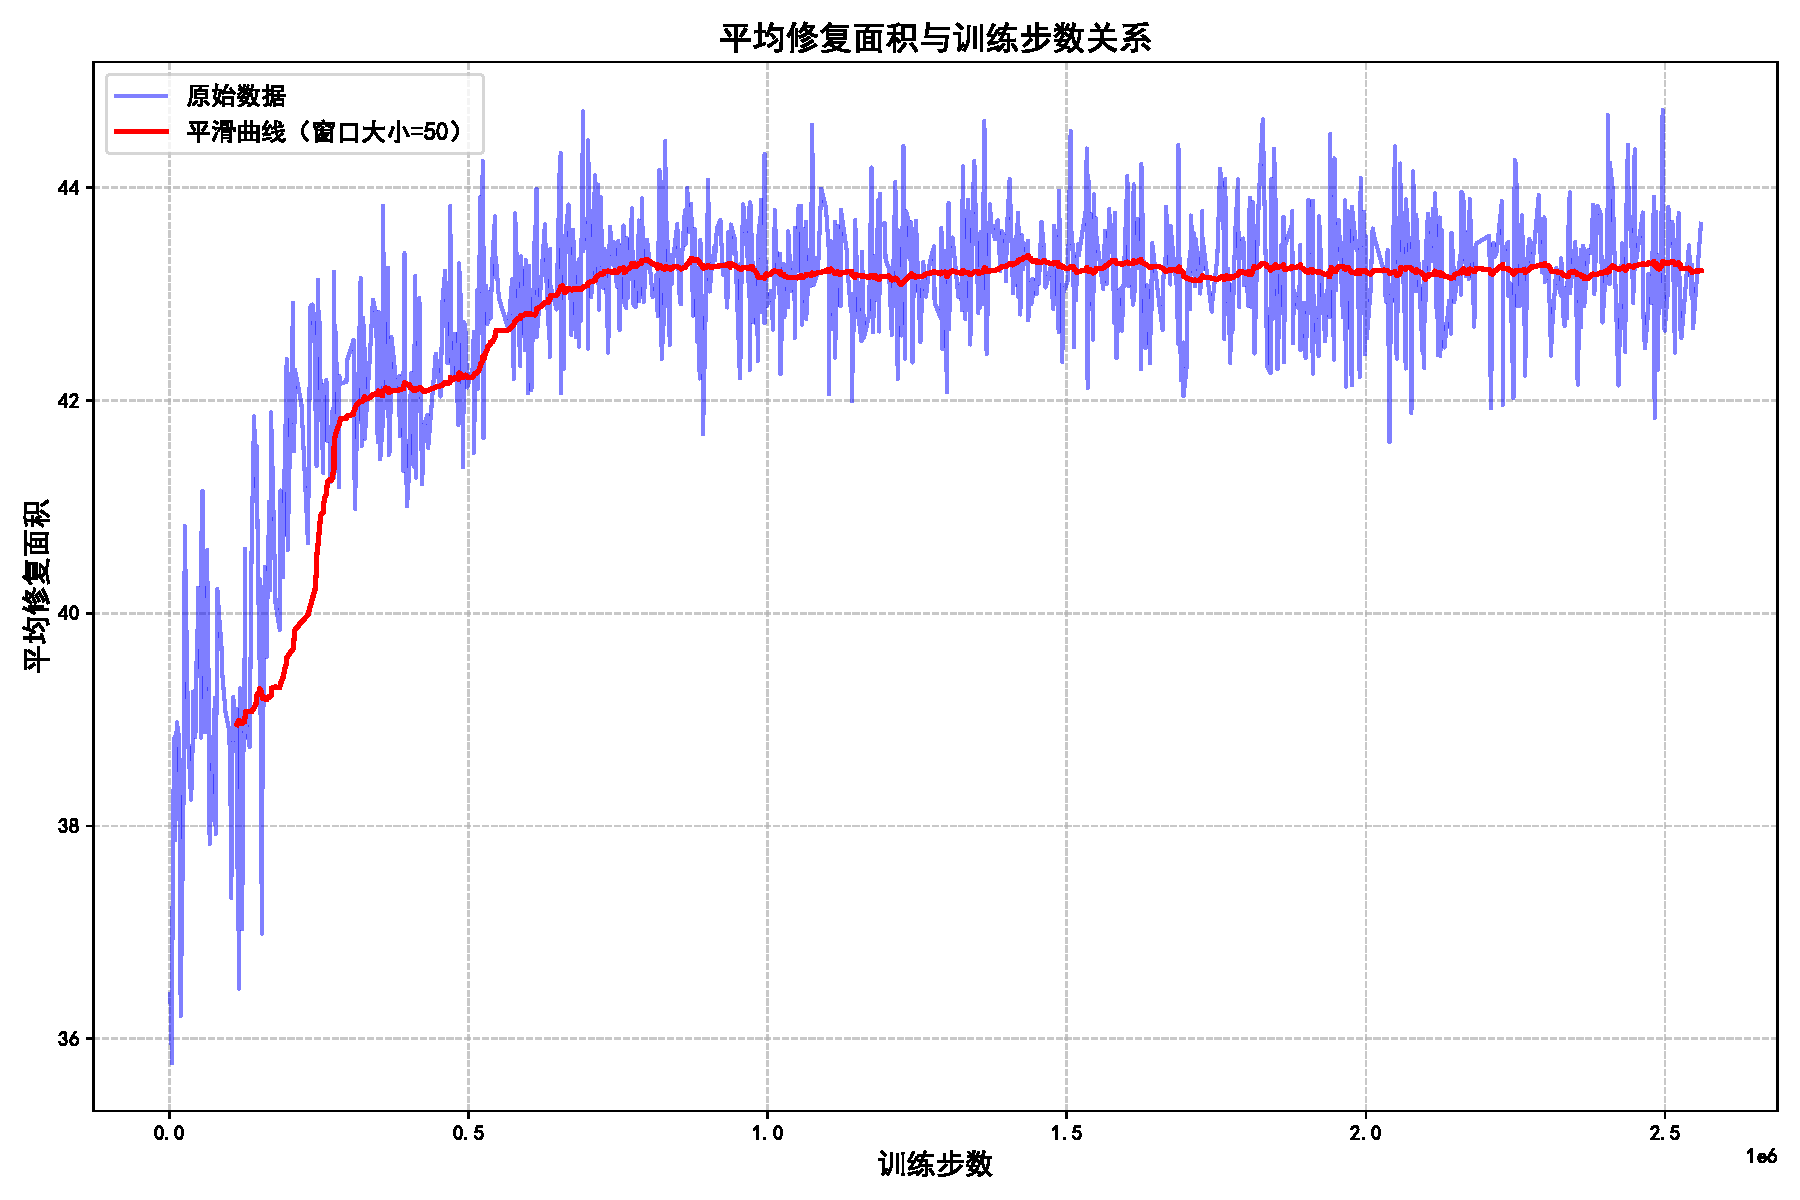
\includegraphics[width=0.6\textwidth]{figures/avg_repair_area_curve.pdf}
	\caption{深度强化学习训练过程中的修复面积变化}
	\label{fig:training_reward_curve}
\end{figure}

如图\ref{fig:training_loss_curve}所示,该图展示了深度强化学习模型在训练过程中的损失函数随迭代轮数的变化趋势,可以看出损失值整体呈下降趋势,表明模型逐步收敛。从曲线可观察到,当训练步数达到约500000步后,损失函数趋于稳定,波动范围显著减小,表明模型已基本收敛。图\ref{fig:training_reward_curve}展示了训练过程中平均修复面积的变化曲线,随着训练的进行,平均修复面积逐步提升,说明模型的决策能力不断增强,能够获得更优的修复方案。同样,在约500000步后,修复面积也达到相对稳定状态,进一步证实了模型的有效收敛。这两个图共同验证了所提出深度强化学习方法在多无人机草原修复任务中的有效性和收敛性。
\begin{figure}[H]
	\centering
	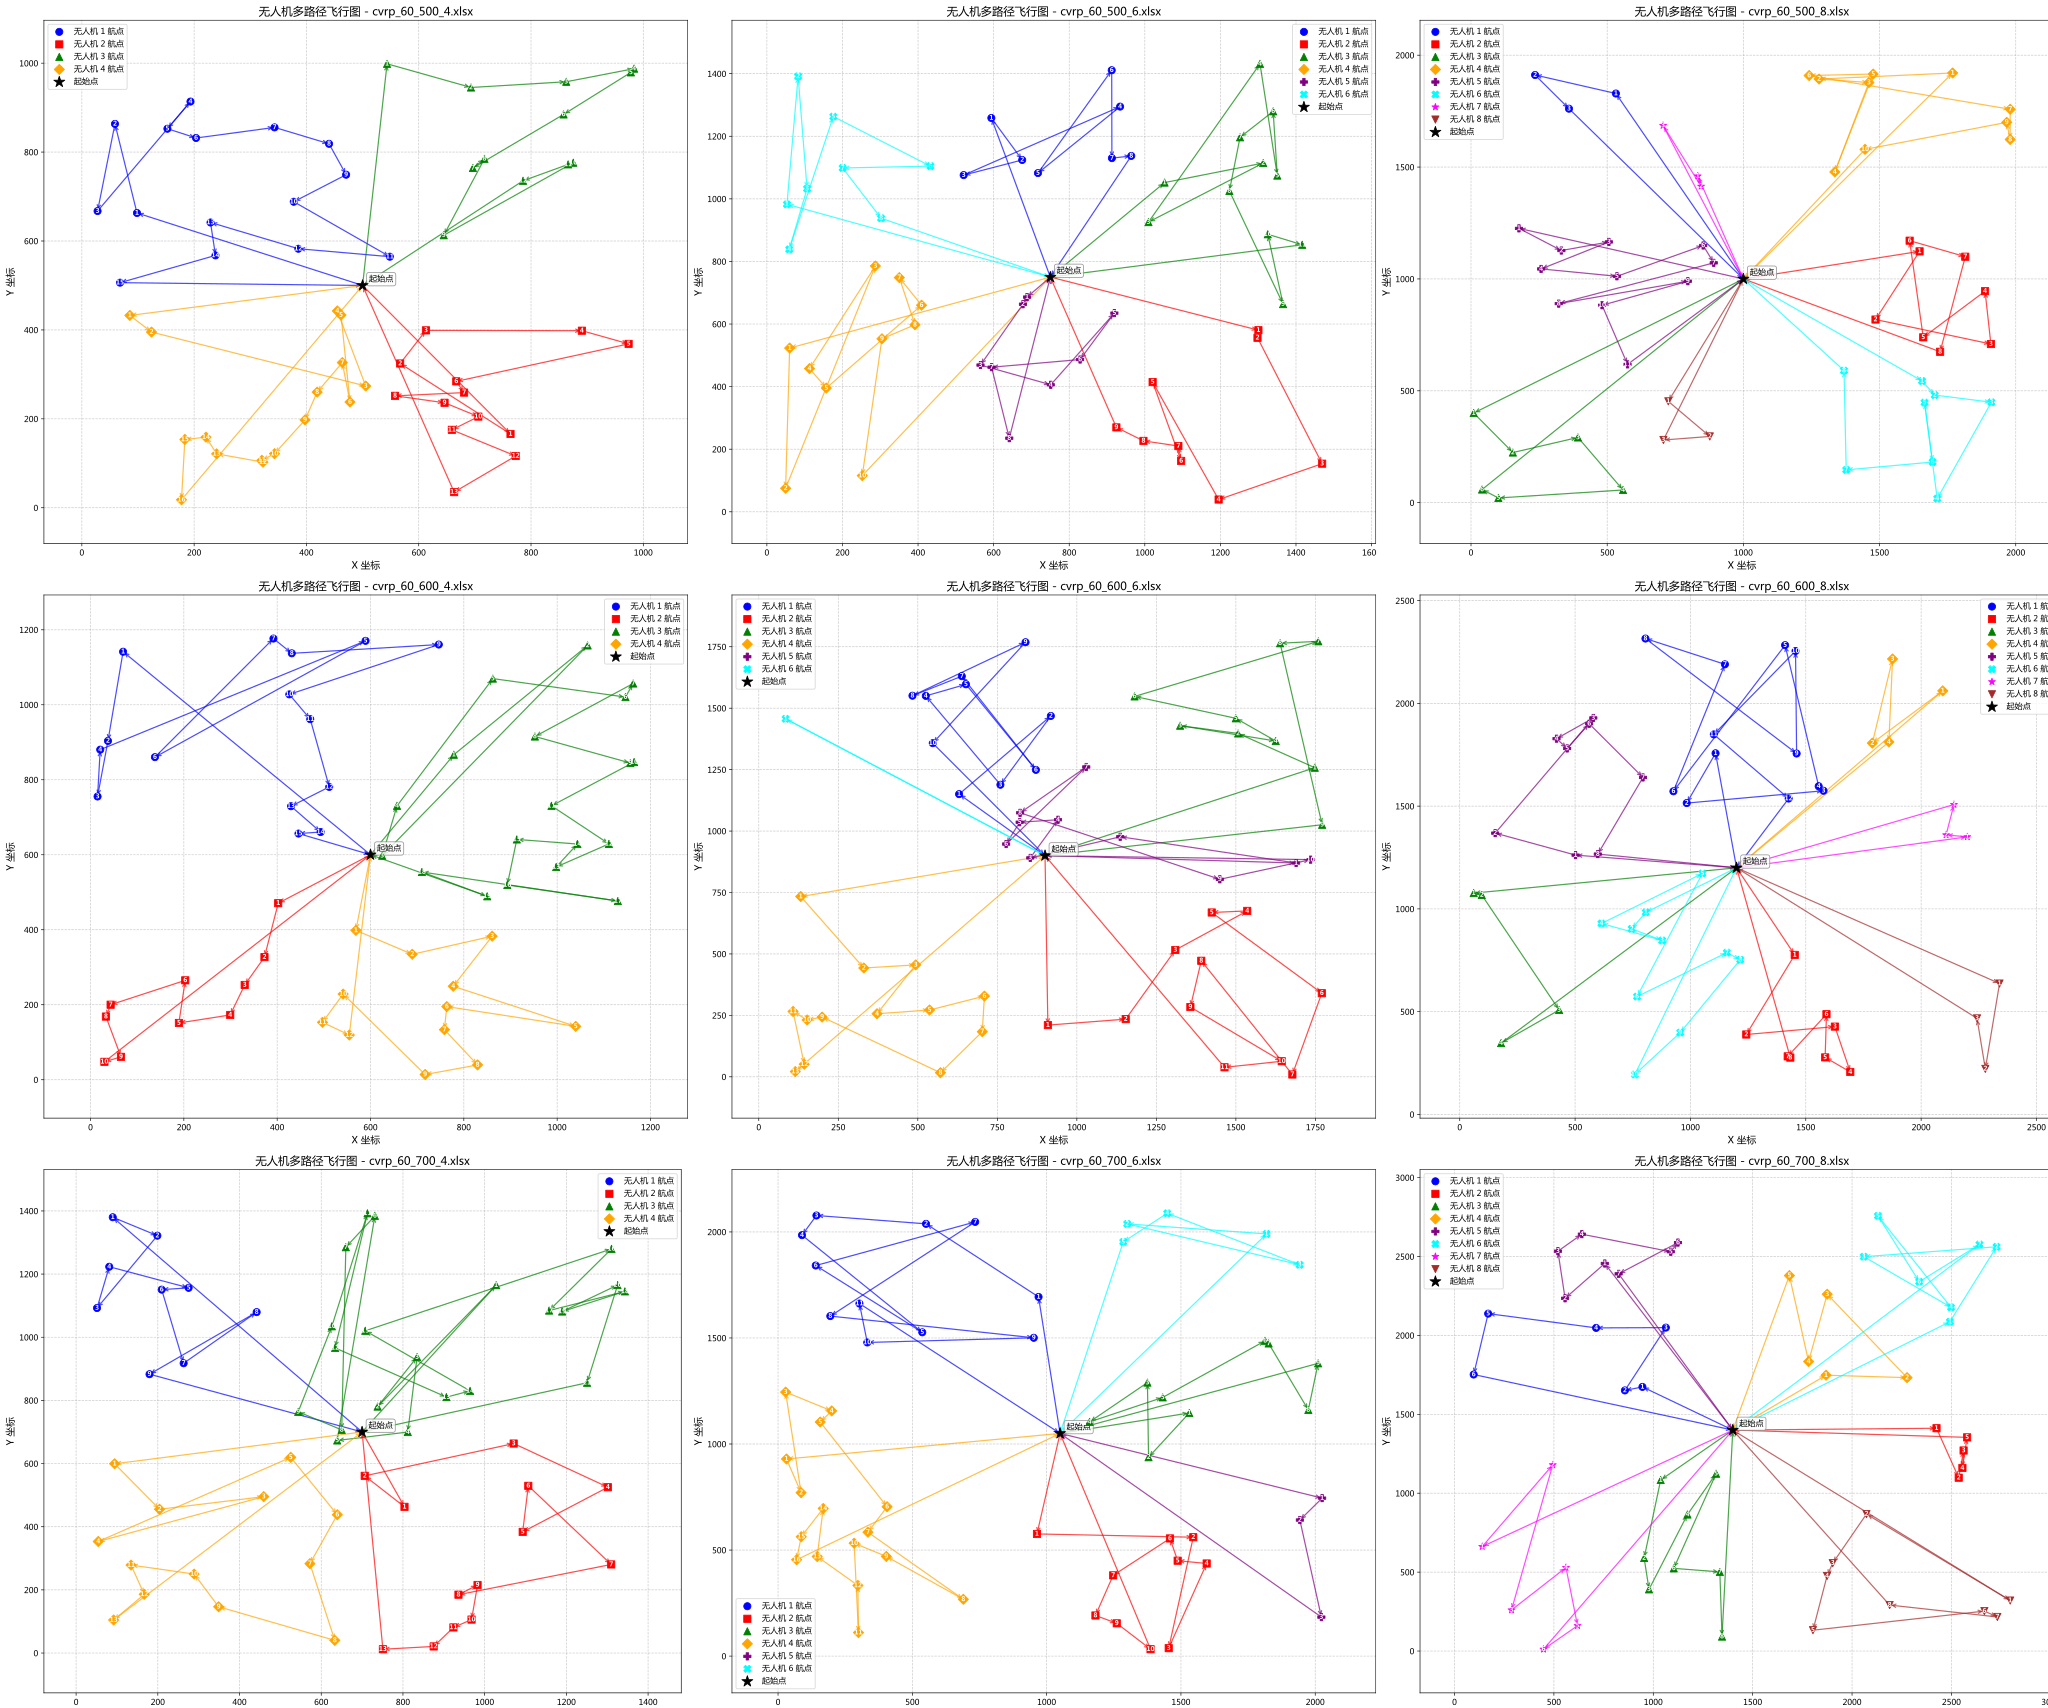
\includegraphics[width=0.99\textwidth]{figures/RL_combined_uav_routes.pdf}
	\caption{基于深度强化学习的多无人机草原修复路径规划}
	\label{fig:RL_combined_uav_routes}
\end{figure}

图\ref{fig:RL_combined_uav_routes}展示了基于深度强化学习方法的多无人机草原修复路径规划结果。可以看到,深度强化学习方法能够为每架无人机分配合理的修复区域,路径交叉较少,任务分配均衡,有效减少了无人机间的干扰。尤其在待修复区域分布密集时,算法能够根据能量约束和区域分布动态优化任务分配,使各无人机负载更为均衡。

\begin{figure}[H]
	\centering
	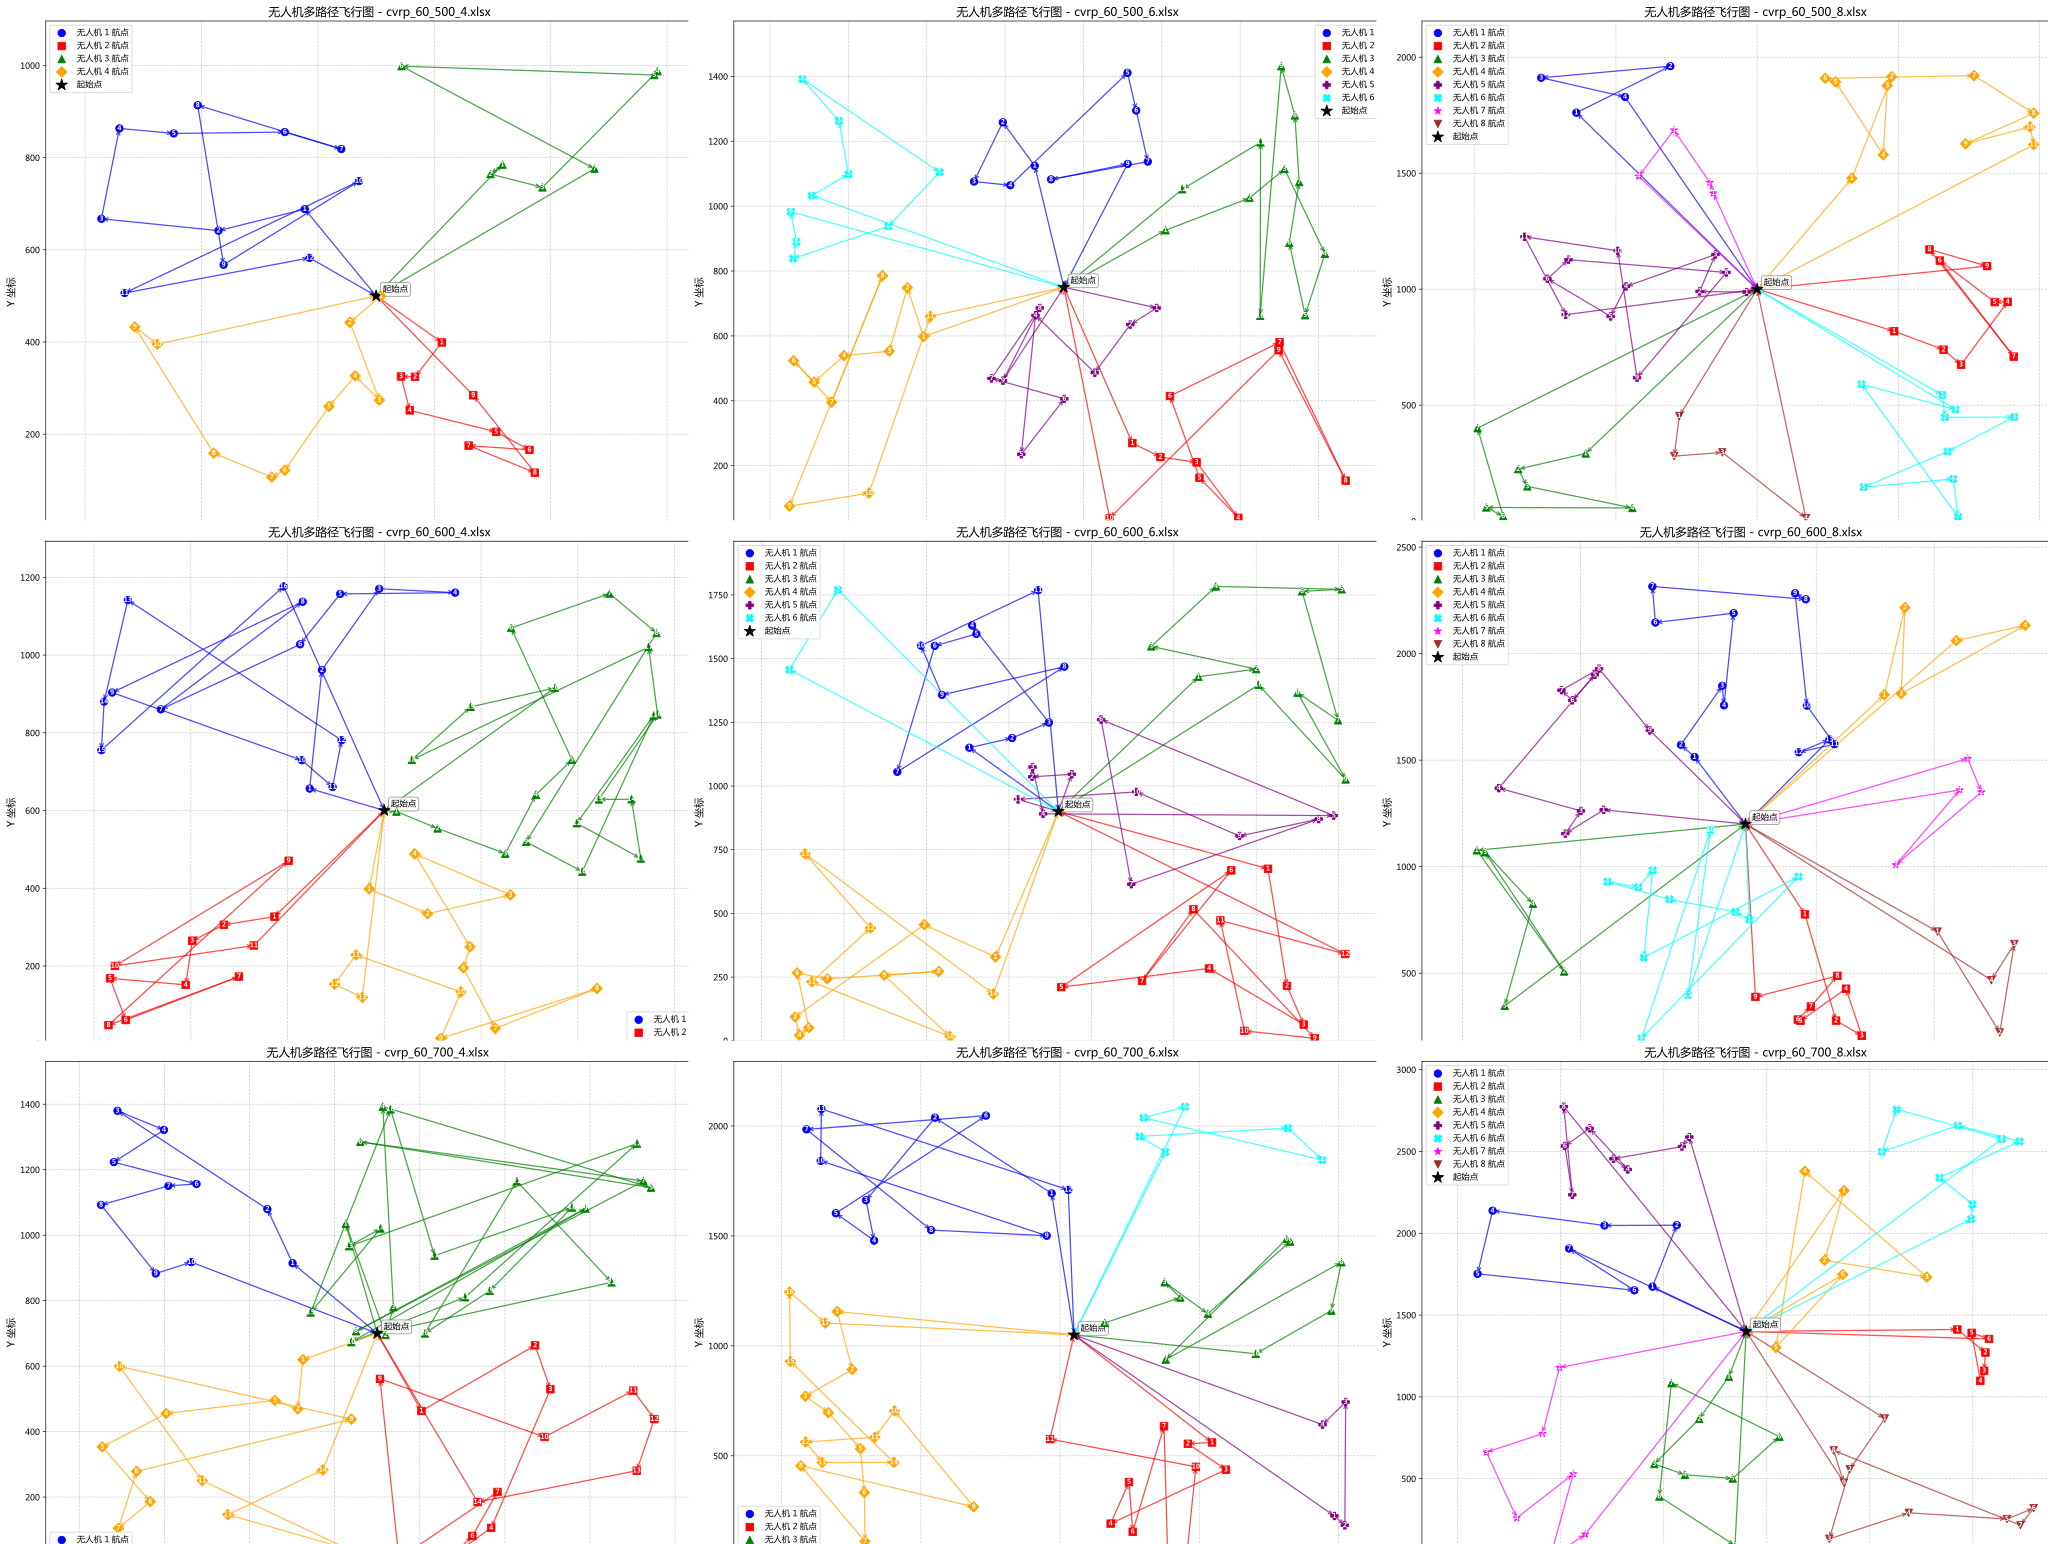
\includegraphics[width=0.99\textwidth]{figures/ILS_combined_uav_routes.pdf}
	\caption{基于迭代局部搜索的多无人机草原修复路径规划}
	\label{fig:ILS_combined_uav_routes}
\end{figure}

图\ref{fig:ILS_combined_uav_routes}为迭代局部搜索方法的多无人机路径规划结果。与深度强化学习方法相比,迭代局部搜索在路径分配上表现出一定局限性,部分无人机路径存在较多长距离飞行和交叉,导致能量消耗增加,任务分配不够灵活。该方法在区域分配上较为机械,难以充分适应区域分布和能耗的动态变化。

通过对比两种方法的路径规划结果可以发现,深度强化学习方法在多无人机协同草原修复任务中表现出更强的自适应能力和优化效果,能够更好地协调任务分配和路径规划,提高修复效率和能量利用率。表\ref{tab:combined_comparison}进一步量化了两种方法在路径长度和修复面积上的性能差异。
\begin{table}[H]
	\centering
	\caption{路径长度与修复面积对比(SA 与 DRL)}
	\small
	\setlength{\tabcolsep}{3.5pt}
	\begin{tabular}{cccc ccc ccc}
		\toprule
		区域数                 & 草原边长                 & 无人机数 &  & \multicolumn{3}{c}{路径长度} & \multicolumn{3}{c}{修复面积}                                       \\
		\cmidrule(lr){5-7} \cmidrule(lr){8-10}
		                    &                      &      &  & DRL                      & SA                       & Gap(\%) & DRL    & SA     & Gap(\%) \\
		\midrule
		\multirow{9}{*}{60} & \multirow{3}{*}{500} & 4    &  & 9396.35                  & 12648.21                 & -25.68  & 267.00 & 194.00 & 37.63   \\
		                    &                      & 6    &  & 21348.69                 & 19110.48                 & 11.71   & 258.00 & 205.00 & 25.85   \\
		                    &                      & 8    &  & 26118.19                 & 27145.66                 & -3.79   & 304.00 & 218.00 & 39.45   \\
		\cmidrule(lr){2-10}
		                    & \multirow{3}{*}{600} & 4    &  & 13339.68                 & 16255.96                 & -17.92  & 271.00 & 223.00 & 21.52   \\
		                    &                      & 6    &  & 26523.73                 & 27174.68                 & -2.39   & 294.00 & 206.00 & 42.72   \\
		                    &                      & 8    &  & 31186.17                 & 31494.13                 & -0.98   & 257.00 & 224.00 & 14.73   \\
		\cmidrule(lr){2-10}
		                    & \multirow{3}{*}{700} & 4    &  & 17622.78                 & 22103.46                 & -20.27  & 282.00 & 291.00 & -3.09   \\
		                    &                      & 6    &  & 28252.23                 & 28539.91                 & -1.01   & 270.00 & 218.00 & 23.85   \\
		                    &                      & 8    &  & 37585.42                 & 36859.35                 & 1.97    & 238.00 & 254.00 & -6.30   \\
		\midrule
		\multirow{9}{*}{80} & \multirow{3}{*}{500} & 4    &  & 10221.88                 & 17217.03                 & -40.60  & 370.00 & 315.00 & 17.46   \\
		                    &                      & 6    &  & 22135.76                 & 25252.45                 & -12.37  & 375.00 & 240.00 & 56.25   \\
		                    &                      & 8    &  & 30491.72                 & 31922.23                 & -4.48   & 306.00 & 267.00 & 14.61   \\
		\cmidrule(lr){2-10}
		                    & \multirow{3}{*}{600} & 4    &  & 15973.03                 & 22825.91                 & -30.02  & 363.00 & 314.00 & 15.61   \\
		                    &                      & 6    &  & 29742.35                 & 28044.73                 & 6.05    & 406.00 & 282.00 & 44.00   \\
		                    &                      & 8    &  & 39943.98                 & 40845.86                 & -2.21   & 399.00 & 269.00 & 48.33   \\
		\cmidrule(lr){2-10}
		                    & \multirow{3}{*}{700} & 4    &  & 22577.68                 & 26113.54                 & -13.56  & 335.00 & 267.00 & 25.47   \\
		                    &                      & 6    &  & 33566.63                 & 34738.58                 & -3.38   & 380.00 & 298.00 & 27.52   \\
		                    &                      & 8    &  & 44308.24                 & 42493.45                 & 4.28    & 355.00 & 311.00 & 14.14   \\
		\bottomrule
	\end{tabular}
	\label{tab:combined_comparison}
\end{table}

由表~\ref{tab:combined_comparison} 可以看出,深度强化学习(DRL)方法在大多数测试场景下均优于模拟退火(SA)算法。在路径长度方面,DRL 在多数情况下实现了更短的总路径,部分场景下路径长度缩短超过 20\%。在修复面积方面,DRL 也表现出显著提升,提升幅度普遍在 15\% 以上,最高可达 56\%。尤其在无人机数量较少或区域分布密集时,DRL 能更好地协调多无人机任务分配,实现更高的修复效率。总体来看,DRL 在路径优化和面积最大化两个方面均优于传统启发式算法,显示出其在复杂多无人机协同任务中的有效性和优势。

% Required packages: \usepackage{booktabs}, \usepackage{float}, \usepackage{multirow}


\chapter{总结与展望}

\section{总结}
我们提出了结合深度强化学习方法求解的多无人机协同草原修复方法,利用深度强化学习的序列决策能力,构建编码器-解码器架构深度神经网络模型,使用强化学习Actor-Critic方法对模型进行训练,无需人为设计即可自动学习出优秀的策略。深度神经网络模型在编码器中的多头注意力层对待修复区域个体特征和待修复区域位置特征进行信息交互,通过自回归解码器输出下一步可能的修复方案。此外,本文还提出了多无人机协同的修复算法,在充分利用已有强化学习方法的基础上进一步优化求解效果。

实验结果表明,本文提出的算法优于基于贪婪策略的双层决策算法,且随着问题规模的增大优势更为明显;相较于贪婪策略,本文提出的单无人机训练、多无人机协同的策略具有更强寻优能力,在规定时间内进一步提升了求解效果,展示出神经网络算法强大的泛化与寻优能力,同时为求解大规模草原修复问题提供了新的思路和方法。

\section{展望}
在仿真结果与分析部分,由于项目时间限制,其中仍有众多方面可以值得扩展研究。例如:在给定的参数范围内,选择更多的启发式算法作为对比算法,从而能对控制算法的性能有更公正的评估。或在本文提出的控制算法框架下,通过控制变量法改变草场规模、无人机初始能量 $E_{max}$ 等参数多次训练神经网络,而后通过大量的随机模拟取最佳、最差及平均等指标,来探讨算法的稳定性。

% \label{sub:国际三线表格}
% \begin{table}[H]
% 	\centering
% 	\caption{二硫化钼纳米管参数}
% 	\begin{tabular}{cccccc} % 控制表格的格式,可以是l,c,r
% 		\toprule
% 		参数 & m  & n  & \tabincell{c}{太长了                     \\换行一下\\原子数}  & 内径 & 长度\\
% 		\midrule
% 		数值 & 15 & 15 & 2880              & 2.3014nm & 9.95nm \\
% 		\bottomrule
% 	\end{tabular}
% 	\label{tbl_mos2_nanotube}
% \end{table}

% 这个注意,有多少列,后面就要有多少个c \footnote{否则会报错:Extra alignment tab has been changed to cr.有什么报错百度一下一般就找到了},这个c表示这一列居中(center),靠左的话:l,右:r;

% 那个label后面的名字自己取,但是不能有重复,是为了引用,比如这样,表格\ref{tbl_mos2_nanotube},方程、图片也是这样引用的,好处是,中间加一个表格导致这个表格的序号变了也没事,你不用再去修改其他地方的引用

% \begin{lstlisting}[language = tex]
% \begin{table}[H]
%     \centering
%     \caption{二硫化钼纳米管参数}
%     \begin{tabular}{cccccc} % 控制表格的格式,可以是l,c,r
%     \toprule
%     参数& m & n & 原子数  & 内径 & 长度\\
%     \midrule
%     数值 & 15 & 15  & 2880 & 2.3014nm & 9.95nm \\
%     \bottomrule
%     \end{tabular}
%     \label{tbl_mos2_nanotube}
% \end{table}
% \end{lstlisting}

% \subsection{换页表格}

% 我是真的没想到有的人表格居然这么长,竟然能有三页。。。。


% \begin{longtable}{cccccc} % 控制表格的格式,可以是l,c,r
% 	\caption{二硫化钼纳米管参数}\label{tbl_mos2_nanotube2} \\
% 	\toprule
% 	参数   & m  & n  & 原子数  & 内径       & 长度         \\
% 	\midrule
% 	数值   & 15 & 15 & 2880 & 2.3014nm & 9.95nm     \\
% 	数值1  & 15 & 15 & 2880 & 2.3014nm & 9.95nm     \\
% 	数值2  & 15 & 15 & 2880 & 2.3014nm & 9.95nm     \\
% 	数值3  & 15 & 15 & 2880 & 2.3014nm & 9.95nm     \\
% 	数值4  & 15 & 15 & 2880 & 2.3014nm & 9.95nm     \\
% 	数值5  & 15 & 15 & 2880 & 2.3014nm & 9.95nm     \\
% 	数值6  & 15 & 15 & 2880 & 2.3014nm & 9.95nm     \\
% 	数值7  & 15 & 15 & 2880 & 2.3014nm & 9.95nm     \\
% 	数值8  & 15 & 15 & 2880 & 2.3014nm & 9.95nm     \\
% 	数值9  & 15 & 15 & 2880 & 2.3014nm & 9.95nm     \\
% 	数值10 & 15 & 15 & 2880 & 2.3014nm & 9.95nm     \\
% 	数值11 & 15 & 15 & 2880 & 2.3014nm & 9.95nm     \\
% 	数值12 & 15 & 15 & 2880 & 2.3014nm & 9.95nm     \\
% 	数值13 & 15 & 15 & 2880 & 2.3014nm & 9.95nm     \\
% 	数值14 & 15 & 15 & 2880 & 2.3014nm & 9.95nm     \\
% 	数值15 & 15 & 15 & 2880 & 2.3014nm & 9.95nm     \\
% 	数值16 & 15 & 15 & 2880 & 2.3014nm & 9.95nm     \\
% 	数值17 & 15 & 15 & 2880 & 2.3014nm & 9.95nm     \\
% 	数值18 & 15 & 15 & 2880 & 2.3014nm & 9.95nm     \\
% 	数值19 & 15 & 15 & 2880 & 2.3014nm & 9.95nm     \\
% 	数值20 & 15 & 15 & 2880 & 2.3014nm & 9.95nm     \\
% 	\bottomrule
% \end{longtable}



% % subsection 国际三线表格 (end)


% \subsection{字体}
% \label{sub:字体}

% \begin{table}[H]
% 	\centering
% 	\caption{字体}
% 	\begin{tabular}{ccccccc} % 控制表格的格式
% 		\toprule
% 		名称 & 加粗           & 倾斜           & 宋体           & 仿宋             & 黑体          \\
% 		\midrule
% 		显示 & \textbf{兰朵儿} & \textit{兰朵儿} & \songti{兰朵儿} & \fangsong{兰朵儿} & \heiti{兰朵儿} \\
% 		显示 & \textbf{ldr} & \textit{ldr} & \songti{ldr} & \fangsong{ldr} & \heiti{ldr} \\
% 		\bottomrule
% 	\end{tabular}
% 	\label{tbl_font}
% \end{table}
% 发现没,中文斜体没有效果的,你可以自定义,这个自己百度吧;中文加粗已经解决了该问题,注意这个文件第四行,开启伪加粗(2020.5.18),可以用bfserie或者textbf但是注意,win上bfserie效果好一些,mac上textbf好一些

% 关于英文新罗马字体的说明:
% 在windows上,引用mathptmx包,正文、公式中的英文就会变成新罗马(Times New Roman)字体,但是mac系统上,没有任何效果,还是默认的罗马字体(和Times New Roman很相似,QR两个单词区分明显),所以我在2.1.3以及之后的模板中加入了以下两个命令:

% \begin{lstlisting}[language = tex]
% \RequirePackage{mathptmx} %加入这条命令会导致花体,mathcal和mathscr完全相同,正常mathcal会花的轻一些。
% \RequirePackage{fontspec} %这一条在windows可有可无,效果相同,但是mac上必须。
% \end{lstlisting}

% 但是mathptmx会导致花体,mathcal和mathscr完全相同,正常mathcal会花的轻一些。


% % subsection 常用的 (end)




% 这一句代表这个图片宽度为一行文本宽度的$\frac{3}{10}$
% \begin{lstlisting}[language = tex]
% width=0.3\textwidth
% \end{lstlisting}



% % subsection 图_并列排 (end)


% \subsection{公式}
% \label{sub:公式}
% 所有的符号都要用美元符号包裹\$,需要用到某一个但是不知道,直接百度,基本上都有
% \begin{table}[H]
% 	\centering
% 	\caption{公式}
% 	\begin{tabular}{cccccccccc} % 控制表格的格式
% 		\toprule
% 		名称 & 分数            & 下角标   & 上角标   & 矢量         & 根号            & 希腊字母     & 点乘      & 叉乘       & 矢量        \\
% 		\midrule
% 		显示 & $\frac{1}{2}$ & $O_2$ & $a^2$ & $\vec{AB}$ & $\sqrt[2]{3}$ & $\theta$ & $\cdot$ & $\times$ & $\vec{a}$ \\

% 		\bottomrule
% 	\end{tabular}
% 	\label{tbl_gs}
% \end{table}

% 但是有时候我们只是正文中想用$MoS_2$,它竟然斜体,不想斜体,我写了个命令,这样用\eqrm{MoS_2},正的吧,常用的命令可以自定义

% \subsection{公式加粗、斜体、字体}

% 公式、字母加粗、字体问题

% \begin{itemize}
% 	\item[1.] 正文 \qquad \quad AHEMoS$\alpha \beta$
% 	\item[2.] 公式 \qquad \quad $AHEMoS \alpha \beta$
% 	\item[3.] mathbf \qquad $\mathbf{AHEMoS\alpha \beta}$
% 	\item[4.] boldsymbol $\boldsymbol{AHEMoS\alpha \beta}$
% 	\item[5.] mathbb \qquad $\mathbb{AHEMoS\alpha \beta}$
% 	      % \item [5. bm] $\bm{AHEMoS\alpha \beta}$
% \end{itemize}

% 这个加粗、斜体、英文字体(含正文和公式内字体),有不同的处理方式,在 .cls 模板文件文件搜索 bm 查看详细说明

% \subsection{一些特殊符号}

% \begin{itemize}
% 	\item 普朗克常量 hslash :$\hslash$
% 	\item 普朗克常量 hbar :$\hbar$
% 	\item 花体 mathscr :$\mathscr{ABCFR}$
% 	\item 花体 mathcal :$\mathcal{ABCFR}$
% 	\item Fraktur字母 :$\mathfrak{ABCFR}$
% \end{itemize}



% % subsection 公式 (end)

% \subsection{左边大括号}
% \label{sub:左边大括号}

% \begin{equation}
% 	\left\{
% 	\begin{array}{rcl}
% 		\vec{e_1} & = \frac{3a}{2} \vec{i} + \frac{\sqrt{3a}}{2} \vec{j} \\
% 		\vec{e_2} & = \frac{3a}{2} \vec{i} - \frac{\sqrt{3a}}{2} \vec{j}
% 	\end{array}
% 	\right.
% 	\label{e1e2}
% \end{equation}

% 注意后面有个方程的编号,如果想取消,把上下的两个$equation$改成$equation*$

% \begin{equation*}
% 	\left\{
% 	\begin{array}{rcl}
% 		\vec{e_1} & = \frac{3a}{2} \vec{i} + \frac{\sqrt{3a}}{2} \vec{j} \\
% 		\vec{e_2} & = \frac{3a}{2} \vec{i} - \frac{\sqrt{3a}}{2} \vec{j}
% 	\end{array}
% 	\right.
% 	\label{e1e2_2}
% \end{equation*}

% % subsection 左边大括号 (end)

% \subsection{复杂公式}
% \label{sub:复杂公式}
% 不会输出的符号,请百度,啥都有

% \begin{equation}
% 	\hat{HQR}=\frac{\epsilon}{2}\hat{\sigma}_{z}-\frac{\Delta}{2}\hat{\sigma}_{x}+\sum_{k}\omega_{k}\hat{b}_{k}^{\dagger}\hat{b}_{k}+\sum_{k}\frac{g_{k}}{2}\hat{\sigma}_{z}(\hat{b}_{k}+\hat{b}_{k}^{\dagger})\label{eq:sbm}
% \end{equation}

% % subsection 复杂公式 (end)


% \subsection{等号对齐站}
% \label{sub:等号对齐站}

% 主要是用这个aligned放在了方程的环境里,等号前面\&控制对齐,每一行后面双斜杠换行

% \begin{equation}
% 	\begin{aligned}
% 		\vec{CH} & = m\cdot \vec{e_1} + n\cdot \vec{e_2}                          \\
% 		         & = \frac{3(m+n)a}{2} \vec{i} + \frac{\sqrt{3}(m-n)a}{2} \vec{j}
% 	\end{aligned}
% 	\label{ch}
% \end{equation}

% % subsection 等号对齐站 (end)

% \subsection{矩阵乘法}
% \label{sub:矩阵乘法}

% 其实就是几个array组合

% \begin{equation}
% 	\left[
% 		\begin{array}{c}
% 			x' \\
% 			y' \\
% 		\end{array}
% 		\right]=
% 	\left[
% 		\begin{array}{cc}
% 			cos \theta   & sin \theta \\
% 			- sin \theta & cos \theta
% 		\end{array}
% 		\right]
% 	\cdot
% 	\left[
% 		\begin{array}{c}
% 			x \\
% 			y \\
% 		\end{array}
% 		\right]
% \end{equation}
% % subsection 矩阵乘法 (end)



% \subsection{附页代码}
% \label{sub:附页代码}
% 可以在LZUThesis.clc里面修改代码格式

% java代码
% \begin{lstlisting}[language = java]
%     System.out.print("兰朵儿")
%     // 试一下中文注释
% \end{lstlisting}


% tex代码
% \begin{lstlisting}[language = tex]
%     width=0.3\textwidth
%     % 注释
% \end{lstlisting}

% python代码
% \begin{lstlisting}[language = python]
%     print("兰朵儿")
%     # 注释
% \end{lstlisting}

% matlab代码有专门的库,但是没必要高亮太多,而且中文适配有问题,直接按照下面这个就可以
% \begin{lstlisting}[language = matlab]
%     display("兰朵儿")
%     % 注释
% \end{lstlisting}

% % subsection 附页代码 (end)

% 伪代码



% \subsection{参考文献}
% \label{sub:参考文献}

% 建议以 web of science 或者文献官网导出的bib为准,请不要使用百度学术、谷歌学术的bib,错误很多,\cite{partl2016, tenne1992polyhedral, tussyadiah2015hotels}。
% 测试不同情况:

% \begin{itemize}
% 	\item 原本科模板\cite{partl2016}
% 	\item 中文“等”测试\cite{partl2021}
% 	\item 大写字母测试\cite{partl2022-2}
% 	\item 连接符号测试\cite{partl2022-3}
% 	\item 中文空格测试\cite{partl2022}
% 	\item 连续显示\cite{partl2021,partl2022-2,partl2022-3}
% 	\item 右上角\cite{partl2016,partl2021,partl2022-2}
% 	\item 中文参考文献 \cite{李刚2006基于动态光谱的脉搏血氧测量精度分析}
% 	\item 标题中特殊符号,bib中双层大括号即可 \cite{PhysRevLett.108.024101}
% 	\item 更多测试(zotero导出)\cite{huangInvestigationThermalRectification2024, wanModulatingThermalConductivity2024, wuThermalRectificationAsymmetric2024, xiaoMOFNanozymemediatedAcetylcholinesterasefree2024}
% \end{itemize}


% 具体怎么用可以百度,我这里告诉你什么可以用,但是具体的,建议百度,更靠谱一些。


% 有参考文献时,编译要经过4步,直接 xelatex --> biber --> xelatex --> xelatex,不然很多问题,vscode配置以后很方便,以下内容放在设置中,重新打开vscode即可,注意命令后面不包含.tex,而是直接 xelatex template 和 biber template

% 修改后可以参考文献自动生成中文等字符\cite{partl2021}\cite{partl2022}\cite{partl2022-2},引用网络资源时链接格式规范化\cite{intelnewsroomIntelUnveils12th2021,wilsonHistoryDevelopmentParallel1994}。


% % subsection 参考文献 (end)

% % section 图标等常用的教程 (end)

% \subsection{引用图、表、公式、章节}

% 为什么要引用?不直接写数字?因为图表顺序变化时,引用的地方会自动变化。每次更加新引用,请四步走编译

% 引用的地方加label,自己写个名字,可以是中文,然后引用的地方如下:

% 如图\ref{fig_ldr}所示

% 如公式\eqref{e1e2}所示,会自动带括号

% 如表\ref{tbl_gs}所示

% 在\ref{sub:参考文献}中已经提及

% % \input{test.tex}

%论文后部
\backmatter
%=======%
%引入参考文献文件
%=======%
\printbib
% \nocite{*} %显示数据库中有的,但是正文没有引用的文献

% \Appendix

% 这里是附录页,附上你的程序或必要的相关知识

% {\bfseries 编译方式:}

\Thanks

在毕业论文完成之际,我想向所有在我学习和研究过程中给予帮助和支持的人表达我诚挚的感谢。

首先,我要衷心感谢我的导师焦栋斌教授。在整个研究过程中,焦老师以其渊博的学识、严谨的治学态度和敏锐的科研洞察力给予我悉心指导。他不仅在学术上为我提供了宝贵的建议和方向,而且在科研思维和方法论上也给了我深刻的启发。没有焦老师的悉心指导和鼓励,我难以完成这项研究工作。

感谢信息科学与工程学院的各位老师,在我本科学习期间传授知识、培养能力,为我打下了坚实的专业基础。特别感谢参与我论文评审和答辩的各位老师,您们的建议和意见使我的论文更加完善。

感谢实验室的师兄师姐和同学们,在日常学习和研究中的讨论和交流,让我受益匪浅。你们的陪伴和支持,使我的研究生活充满乐趣和动力。

感谢我的家人,是你们无条件的支持和理解,让我能够专心致志地投入学习和研究。你们是我坚强的后盾和不断前行的动力源泉。

最后,感谢所有在我成长道路上给予过帮助的人,正是因为有了你们的支持与鼓励,我才能顺利完成学业,迎接人生的新挑战。

\Grade %这一句才是成绩页,上面是填写

\end{document}
